\documentclass{book}
\usepackage[a4paper,top=2.5cm,bottom=2.5cm,left=2.5cm,right=2.5cm]{geometry}
\usepackage{makeidx}
\usepackage{natbib}
\usepackage{graphicx}
\usepackage{multicol}
\usepackage{float}
\usepackage{listings}
\usepackage{color}
\usepackage{ifthen}
\usepackage[table]{xcolor}
\usepackage{textcomp}
\usepackage{alltt}
\usepackage{ifpdf}
\ifpdf
\usepackage[pdftex,
            pagebackref=true,
            colorlinks=true,
            linkcolor=blue,
            unicode
           ]{hyperref}
\else
\usepackage[ps2pdf,
            pagebackref=true,
            colorlinks=true,
            linkcolor=blue,
            unicode
           ]{hyperref}
\usepackage{pspicture}
\fi
\usepackage[utf8]{inputenc}
\usepackage[spanish]{babel}
\usepackage{mathptmx}
\usepackage[scaled=.90]{helvet}
\usepackage{courier}
\usepackage{sectsty}
\usepackage{amssymb}
\usepackage[titles]{tocloft}
\usepackage{doxygen}
\lstset{language=C++,inputencoding=utf8,basicstyle=\footnotesize,breaklines=true,breakatwhitespace=true,tabsize=2,numbers=left }
\makeindex
\setcounter{tocdepth}{3}
\renewcommand{\footrulewidth}{0.4pt}
\renewcommand{\familydefault}{\sfdefault}
\hfuzz=15pt
\setlength{\emergencystretch}{15pt}
\hbadness=750
\tolerance=750
\begin{document}
\hypersetup{pageanchor=false,citecolor=blue}
\begin{titlepage}
\vspace*{7cm}
\begin{center}
{\Large P\-R\-A\-C\-T\-I\-C\-A de P\-R\-O2. Reproducción en el laboratorio \\[1ex]\large versión 26-\/mayo-\/2014 }\\
\vspace*{1cm}
{\large Generado por Doxygen 1.8.2}\\
\vspace*{0.5cm}
{\small Viernes, 23 de Mayo de 2014 17:58:20}\\
\end{center}
\end{titlepage}
\clearemptydoublepage
\pagenumbering{roman}
\tableofcontents
\clearemptydoublepage
\pagenumbering{arabic}
\hypersetup{pageanchor=true,citecolor=blue}
\chapter{P\-R\-A\-C\-T\-I\-C\-A de P\-R\-O2.}
\label{index}\hypertarget{index}{}P\-R\-I\-M\-A\-V\-E\-R\-A 2014.

Los científicos de un laboratorio de investigación biológica desean llevar a cabo una serie de experimentos para estudiar el ciclo de vida de una especie de organismos celulares sencillos.

Los científicos del laboratorio jugaran con organismos de células estructurados en forma de árbol. Cada célula del organismo contiene dos atributos\-: el identificador (un número natural mayor que zero) y la actividad, ya que una célula puede ser o bien activa (true) o pasiva (false).

Por cada experimento que realizen recibiran al inicio unos N organismos iniciales, con un M maximo organismos por el experimento, dónde M siempre será mas grande estrictamente que N.

Entonces a partir de estos N organismos iniciales dispondran de cinco opciones para poder trabajar con ellos\-:

Opción 1. Aplicar un estirón a un subconjunto de organismos.

Opción 2. Aplicar un recorte a un subconjunto de organismos.

Opción 3. Aplicar una ronda de reproducción en el experimento.

Opción 4. Obtener el ranking de reproducción de todos los organismos existentes.

Opción 5. Consultar el estado de un subconjunto de organismos.

Después de todo ello, el experimento finalizará cuando o bien lo finalizen manualmente, o todos los organismos hayan muerto o se haya alcanzado el máximo permitido. 
\chapter{Índice de clases}
\section{Lista de clases}
Lista de las clases, estructuras, uniones e interfaces con una breve descripción\-:\begin{DoxyCompactList}
\item\contentsline{section}{\hyperlink{class_celula}{Celula} \\*Representa una celula con atributos identificador y actividad }{\pageref{class_celula}}{}
\item\contentsline{section}{\hyperlink{class_experiment}{Experiment} \\*Representa un experiment como un conjunto de organismes }{\pageref{class_experiment}}{}
\item\contentsline{section}{\hyperlink{class_organisme}{Organisme} \\*Representa un organisme como arbol de celulas, el máximo identificador y si puede crecer o no }{\pageref{class_organisme}}{}
\item\contentsline{section}{\hyperlink{class_ranking}{Ranking} \\*Representa un ranking de todos los organismos del experiment }{\pageref{class_ranking}}{}
\end{DoxyCompactList}

\chapter{Indice de archivos}
\section{Lista de archivos}
Lista de todos los archivos con descripciones breves\-:\begin{DoxyCompactList}
\item\contentsline{section}{\hyperlink{_celula_8cpp}{Celula.\-cpp} \\*Código de la clase \hyperlink{class_celula}{Celula} }{\pageref{_celula_8cpp}}{}
\item\contentsline{section}{\hyperlink{_celula_8hpp}{Celula.\-hpp} \\*Especificación de la clase \hyperlink{class_celula}{Celula} }{\pageref{_celula_8hpp}}{}
\item\contentsline{section}{\hyperlink{_experiment_8cpp}{Experiment.\-cpp} \\*Código de la clase \hyperlink{class_experiment}{Experiment} }{\pageref{_experiment_8cpp}}{}
\item\contentsline{section}{\hyperlink{_experiment_8hpp}{Experiment.\-hpp} \\*Especificación de la clase \hyperlink{class_experiment}{Experiment} }{\pageref{_experiment_8hpp}}{}
\item\contentsline{section}{\hyperlink{_organisme_8cpp}{Organisme.\-cpp} \\*Código de la clase \hyperlink{class_organisme}{Organisme} }{\pageref{_organisme_8cpp}}{}
\item\contentsline{section}{\hyperlink{_organisme_8hpp}{Organisme.\-hpp} \\*Especificación de la clase \hyperlink{class_organisme}{Organisme} }{\pageref{_organisme_8hpp}}{}
\item\contentsline{section}{\hyperlink{pro2_8cpp}{pro2.\-cpp} \\*Programa principal para la P\-R\-A\-C\-T\-I\-C\-A de P\-R\-O2 }{\pageref{pro2_8cpp}}{}
\item\contentsline{section}{\hyperlink{_ranking_8cpp}{Ranking.\-cpp} \\*Código de la clase \hyperlink{class_ranking}{Ranking} }{\pageref{_ranking_8cpp}}{}
\item\contentsline{section}{\hyperlink{_ranking_8hpp}{Ranking.\-hpp} \\*Especificación de la clase \hyperlink{class_ranking}{Ranking} }{\pageref{_ranking_8hpp}}{}
\end{DoxyCompactList}

\chapter{Documentación de las clases}
\hypertarget{class_celula}{\section{Referencia de la Clase Celula}
\label{class_celula}\index{Celula@{Celula}}
}


Representa una celula con atributos identificador y actividad.  


\subsection*{Métodos públicos}
\begin{DoxyCompactItemize}
\item 
\hyperlink{class_celula_a3c5017fbcec8cb564acc666aa7e21206}{Celula} ()
\begin{DoxyCompactList}\small\item\em Creadora por defecto. \end{DoxyCompactList}\item 
\hyperlink{class_celula_a9fac2a026e4205b7ca6f9c582d2bf5c0}{Celula} (int iden, bool activ)
\begin{DoxyCompactList}\small\item\em Creadora con valores concretos. \end{DoxyCompactList}\item 
void \hyperlink{class_celula_ad8549ea461baa63298e8548691a270e2}{modificar\-\_\-id} (int iden)
\begin{DoxyCompactList}\small\item\em Modificadora del identificador. \end{DoxyCompactList}\item 
void \hyperlink{class_celula_a5bccaca548ef9f6c06e06a64265fabe3}{modificar\-\_\-activa} (bool activ)
\begin{DoxyCompactList}\small\item\em Modificadora de la actividad. \end{DoxyCompactList}\item 
int \hyperlink{class_celula_adfe788cb113f6e8dcf9def377a248255}{consultar\-\_\-id} () const 
\begin{DoxyCompactList}\small\item\em Consultora del identificador. \end{DoxyCompactList}\item 
bool \hyperlink{class_celula_a750270ff8277447af6cc3a122d585aab}{consultar\-\_\-activa} () const 
\begin{DoxyCompactList}\small\item\em Consultora de la actividad. \end{DoxyCompactList}\item 
void \hyperlink{class_celula_a975bfa82da9b298581d0df62102a394c}{leer\-\_\-celula} ()
\begin{DoxyCompactList}\small\item\em Operación de lectura. \end{DoxyCompactList}\item 
void \hyperlink{class_celula_ae476459eced4dd9982795efdc9a1c5fd}{escribir\-\_\-celula} () const 
\begin{DoxyCompactList}\small\item\em Operación de escritura. \end{DoxyCompactList}\end{DoxyCompactItemize}
\subsection*{Atributos privados}
\begin{DoxyCompactItemize}
\item 
int \hyperlink{class_celula_a0984a8b3deeed4979ed6f6141edc3c0c}{id}
\begin{DoxyCompactList}\small\item\em Identificador de la celula. \end{DoxyCompactList}\item 
bool \hyperlink{class_celula_a22ec0fe5fde605b5b3067acde093a3f7}{activa}
\begin{DoxyCompactList}\small\item\em Indica si es activa (true) o pasiva (false) \end{DoxyCompactList}\end{DoxyCompactItemize}


\subsection{Descripción detallada}
Representa una celula con atributos identificador y actividad. 

Definición en la línea 14 del archivo Celula.\-hpp.



\subsection{Documentación del constructor y destructor}
\hypertarget{class_celula_a3c5017fbcec8cb564acc666aa7e21206}{\index{Celula@{Celula}!Celula@{Celula}}
\index{Celula@{Celula}!Celula@{Celula}}
\subsubsection[{Celula}]{\setlength{\rightskip}{0pt plus 5cm}Celula\-::\-Celula (
\begin{DoxyParamCaption}
{}
\end{DoxyParamCaption}
)}}\label{class_celula_a3c5017fbcec8cb564acc666aa7e21206}


Creadora por defecto. 

Se ejecuta automáticamente al declarar una celula \begin{DoxyPrecond}{Precondición}
cierto 
\end{DoxyPrecond}
\begin{DoxyPostcond}{Postcondición}
El resultado es una celula sin valores determinados para sus atributos 
\end{DoxyPostcond}


Definición en la línea 9 del archivo Celula.\-cpp.


\begin{DoxyCode}
\{\}
\end{DoxyCode}
\hypertarget{class_celula_a9fac2a026e4205b7ca6f9c582d2bf5c0}{\index{Celula@{Celula}!Celula@{Celula}}
\index{Celula@{Celula}!Celula@{Celula}}
\subsubsection[{Celula}]{\setlength{\rightskip}{0pt plus 5cm}Celula\-::\-Celula (
\begin{DoxyParamCaption}
\item[{int}]{iden, }
\item[{bool}]{activ}
\end{DoxyParamCaption}
)}}\label{class_celula_a9fac2a026e4205b7ca6f9c582d2bf5c0}


Creadora con valores concretos. 

\begin{DoxyPrecond}{Precondición}
iden $>$ 0 
\end{DoxyPrecond}
\begin{DoxyPostcond}{Postcondición}
El resultado es una celula con identificador \char`\"{}iden\char`\"{} y actividad \char`\"{}activ\char`\"{} 
\end{DoxyPostcond}


Definición en la línea 11 del archivo Celula.\-cpp.


\begin{DoxyCode}
\{
    \textcolor{keywordtype}{id} = iden;
    \hyperlink{class_celula_a22ec0fe5fde605b5b3067acde093a3f7}{activa} = activ;
\}
\end{DoxyCode}


\subsection{Documentación de las funciones miembro}
\hypertarget{class_celula_ad8549ea461baa63298e8548691a270e2}{\index{Celula@{Celula}!modificar\-\_\-id@{modificar\-\_\-id}}
\index{modificar\-\_\-id@{modificar\-\_\-id}!Celula@{Celula}}
\subsubsection[{modificar\-\_\-id}]{\setlength{\rightskip}{0pt plus 5cm}void Celula\-::modificar\-\_\-id (
\begin{DoxyParamCaption}
\item[{int}]{iden}
\end{DoxyParamCaption}
)}}\label{class_celula_ad8549ea461baa63298e8548691a270e2}


Modificadora del identificador. 

\begin{DoxyPrecond}{Precondición}
iden $>$ 0 
\end{DoxyPrecond}
\begin{DoxyPostcond}{Postcondición}
El parámetro implícito pasa a tener identificador \char`\"{}iden\char`\"{} 
\end{DoxyPostcond}


Definición en la línea 19 del archivo Celula.\-cpp.


\begin{DoxyCode}
\{
    \textcolor{keywordtype}{id} = iden;
\}
\end{DoxyCode}
\hypertarget{class_celula_a5bccaca548ef9f6c06e06a64265fabe3}{\index{Celula@{Celula}!modificar\-\_\-activa@{modificar\-\_\-activa}}
\index{modificar\-\_\-activa@{modificar\-\_\-activa}!Celula@{Celula}}
\subsubsection[{modificar\-\_\-activa}]{\setlength{\rightskip}{0pt plus 5cm}void Celula\-::modificar\-\_\-activa (
\begin{DoxyParamCaption}
\item[{bool}]{activ}
\end{DoxyParamCaption}
)}}\label{class_celula_a5bccaca548ef9f6c06e06a64265fabe3}


Modificadora de la actividad. 

\begin{DoxyPrecond}{Precondición}
cierto 
\end{DoxyPrecond}
\begin{DoxyPostcond}{Postcondición}
El parámetro implícito pasa a tener actividad \char`\"{}activ\char`\"{} 
\end{DoxyPostcond}


Definición en la línea 24 del archivo Celula.\-cpp.


\begin{DoxyCode}
\{
    \hyperlink{class_celula_a22ec0fe5fde605b5b3067acde093a3f7}{activa} = activ;
\}
\end{DoxyCode}
\hypertarget{class_celula_adfe788cb113f6e8dcf9def377a248255}{\index{Celula@{Celula}!consultar\-\_\-id@{consultar\-\_\-id}}
\index{consultar\-\_\-id@{consultar\-\_\-id}!Celula@{Celula}}
\subsubsection[{consultar\-\_\-id}]{\setlength{\rightskip}{0pt plus 5cm}int Celula\-::consultar\-\_\-id (
\begin{DoxyParamCaption}
{}
\end{DoxyParamCaption}
) const}}\label{class_celula_adfe788cb113f6e8dcf9def377a248255}


Consultora del identificador. 

\begin{DoxyPrecond}{Precondición}
cierto 
\end{DoxyPrecond}
\begin{DoxyPostcond}{Postcondición}
El resultado es el identificador del parámetro implícito 
\end{DoxyPostcond}


Definición en la línea 31 del archivo Celula.\-cpp.


\begin{DoxyCode}
\{
    \textcolor{keywordflow}{return} \hyperlink{class_celula_a0984a8b3deeed4979ed6f6141edc3c0c}{id};
\}
\end{DoxyCode}
\hypertarget{class_celula_a750270ff8277447af6cc3a122d585aab}{\index{Celula@{Celula}!consultar\-\_\-activa@{consultar\-\_\-activa}}
\index{consultar\-\_\-activa@{consultar\-\_\-activa}!Celula@{Celula}}
\subsubsection[{consultar\-\_\-activa}]{\setlength{\rightskip}{0pt plus 5cm}bool Celula\-::consultar\-\_\-activa (
\begin{DoxyParamCaption}
{}
\end{DoxyParamCaption}
) const}}\label{class_celula_a750270ff8277447af6cc3a122d585aab}


Consultora de la actividad. 

\begin{DoxyPrecond}{Precondición}
cierto 
\end{DoxyPrecond}
\begin{DoxyPostcond}{Postcondición}
El resultado es la actividad del parámetro implícito 
\end{DoxyPostcond}


Definición en la línea 36 del archivo Celula.\-cpp.


\begin{DoxyCode}
\{
    \textcolor{keywordflow}{return} \hyperlink{class_celula_a22ec0fe5fde605b5b3067acde093a3f7}{activa};
\}
\end{DoxyCode}
\hypertarget{class_celula_a975bfa82da9b298581d0df62102a394c}{\index{Celula@{Celula}!leer\-\_\-celula@{leer\-\_\-celula}}
\index{leer\-\_\-celula@{leer\-\_\-celula}!Celula@{Celula}}
\subsubsection[{leer\-\_\-celula}]{\setlength{\rightskip}{0pt plus 5cm}void Celula\-::leer\-\_\-celula (
\begin{DoxyParamCaption}
{}
\end{DoxyParamCaption}
)}}\label{class_celula_a975bfa82da9b298581d0df62102a394c}


Operación de lectura. 

\begin{DoxyPrecond}{Precondición}
cierto 
\end{DoxyPrecond}
\begin{DoxyPostcond}{Postcondición}
Se han leido los atributos del parámetro implícito en el canal standard de entrada. 
\end{DoxyPostcond}


Definición en la línea 43 del archivo Celula.\-cpp.


\begin{DoxyCode}
\{
    \textcolor{keywordtype}{id} = readint();
    \textcolor{keywordflow}{if} (\textcolor{keywordtype}{id} != 0) \hyperlink{class_celula_a22ec0fe5fde605b5b3067acde093a3f7}{activa} = readbool();
\}
\end{DoxyCode}
\hypertarget{class_celula_ae476459eced4dd9982795efdc9a1c5fd}{\index{Celula@{Celula}!escribir\-\_\-celula@{escribir\-\_\-celula}}
\index{escribir\-\_\-celula@{escribir\-\_\-celula}!Celula@{Celula}}
\subsubsection[{escribir\-\_\-celula}]{\setlength{\rightskip}{0pt plus 5cm}void Celula\-::escribir\-\_\-celula (
\begin{DoxyParamCaption}
{}
\end{DoxyParamCaption}
) const}}\label{class_celula_ae476459eced4dd9982795efdc9a1c5fd}


Operación de escritura. 

\begin{DoxyPrecond}{Precondición}
cierto 
\end{DoxyPrecond}
\begin{DoxyPostcond}{Postcondición}
Se han escrito los atributos del parámetro implícito en el canal standard de salida. 
\end{DoxyPostcond}


Definición en la línea 51 del archivo Celula.\-cpp.


\begin{DoxyCode}
\{
    cout << \textcolor{keywordtype}{id} << \textcolor{stringliteral}{" "};
    \textcolor{keywordflow}{if} (\hyperlink{class_celula_a22ec0fe5fde605b5b3067acde093a3f7}{activa}) cout << \textcolor{stringliteral}{"1 "};
    \textcolor{keywordflow}{else} cout << \textcolor{stringliteral}{"-1 "};
\}
\end{DoxyCode}


\subsection{Documentación de los datos miembro}
\hypertarget{class_celula_a0984a8b3deeed4979ed6f6141edc3c0c}{\index{Celula@{Celula}!id@{id}}
\index{id@{id}!Celula@{Celula}}
\subsubsection[{id}]{\setlength{\rightskip}{0pt plus 5cm}int Celula\-::id\hspace{0.3cm}{\ttfamily [private]}}}\label{class_celula_a0984a8b3deeed4979ed6f6141edc3c0c}


Identificador de la celula. 



Definición en la línea 18 del archivo Celula.\-hpp.

\hypertarget{class_celula_a22ec0fe5fde605b5b3067acde093a3f7}{\index{Celula@{Celula}!activa@{activa}}
\index{activa@{activa}!Celula@{Celula}}
\subsubsection[{activa}]{\setlength{\rightskip}{0pt plus 5cm}bool Celula\-::activa\hspace{0.3cm}{\ttfamily [private]}}}\label{class_celula_a22ec0fe5fde605b5b3067acde093a3f7}


Indica si es activa (true) o pasiva (false) 



Definición en la línea 20 del archivo Celula.\-hpp.



La documentación para esta clase fue generada a partir de los siguientes ficheros\-:\begin{DoxyCompactItemize}
\item 
\hyperlink{_celula_8hpp}{Celula.\-hpp}\item 
\hyperlink{_celula_8cpp}{Celula.\-cpp}\end{DoxyCompactItemize}

\hypertarget{class_experiment}{\section{Referencia de la Clase Experiment}
\label{class_experiment}\index{Experiment@{Experiment}}
}


Representa un experiment como un conjunto de organismes.  


\subsection*{Métodos públicos}
\begin{DoxyCompactItemize}
\item 
\hyperlink{class_experiment_a303e6a05d99f403ff4793495a2fbff58}{Experiment} ()
\begin{DoxyCompactList}\small\item\em Creadora por defecto. \end{DoxyCompactList}\item 
\hyperlink{class_experiment_a29118152cb5d4d3197764ed9baa998b4}{Experiment} (int m)
\begin{DoxyCompactList}\small\item\em Creadora con tamaño predeterminado. \end{DoxyCompactList}\item 
int \hyperlink{class_experiment_af88536a26e7e074a30edae50e86e4550}{reproduccion} (\hyperlink{class_ranking}{Ranking} \&R)
\begin{DoxyCompactList}\small\item\em Ronda de reproducción de organismes. \end{DoxyCompactList}\item 
void \hyperlink{class_experiment_a2658473f47b7df935fb1e2b48159824d}{estiron} (int x)
\begin{DoxyCompactList}\small\item\em Crecimiento de un organismo. \end{DoxyCompactList}\item 
void \hyperlink{class_experiment_a1c3d6fabc67e6d9f2a3f72e7845f5988}{recorte} (int x)
\begin{DoxyCompactList}\small\item\em Decrecimiento de un organismo. \end{DoxyCompactList}\item 
int \hyperlink{class_experiment_a32df1020a5b5e27949bd2bce272a36d9}{tamano} () const 
\begin{DoxyCompactList}\small\item\em Consultora de tamaño. \end{DoxyCompactList}\item 
int \hyperlink{class_experiment_a333c9c8084c76beb6b8848b8f2efec25}{tamano\-\_\-maximo} () const 
\begin{DoxyCompactList}\small\item\em Consultora de tamaño máximo. \end{DoxyCompactList}\item 
int \hyperlink{class_experiment_a1f1307d2224b32b4b642b7e545f655f6}{consultar\-\_\-vius} () const 
\begin{DoxyCompactList}\small\item\em Consultora de organismos vivos. \end{DoxyCompactList}\item 
bool \hyperlink{class_experiment_af08a77ada723ccaaf6476a3c1331261c}{muerto} () const 
\begin{DoxyCompactList}\small\item\em Consultora de muerte de todos los organismos. \end{DoxyCompactList}\item 
void \hyperlink{class_experiment_a02185fb874c9439991a68ab436d084bf}{leer\-\_\-experiment} (int marca)
\begin{DoxyCompactList}\small\item\em Operación de lectura. \end{DoxyCompactList}\item 
void \hyperlink{class_experiment_ac2ae9b839376abeac7f65aaea846e70e}{escribir\-\_\-organisme} (int x)
\begin{DoxyCompactList}\small\item\em Operación de escritura de un organisme del experiment. \end{DoxyCompactList}\item 
void \hyperlink{class_experiment_a7306fc6afaffe4783774d58e05efc10c}{escribir\-\_\-ultims} (int x)
\begin{DoxyCompactList}\small\item\em Operación de escritura de los ultimos hijos de la ronda. \end{DoxyCompactList}\end{DoxyCompactItemize}
\subsection*{Atributos privados}
\begin{DoxyCompactItemize}
\item 
int \hyperlink{class_experiment_a329359965b798fa1023b1b29d6ccf832}{M\-A\-X\-O\-R\-G\-A\-N\-I\-S\-M\-E\-S}
\begin{DoxyCompactList}\small\item\em Indica los maximos organismos posibles del experiment. \end{DoxyCompactList}\item 
int \hyperlink{class_experiment_aec56e0b0a0cda4d67ce25a0921d9ebf7}{mida}
\begin{DoxyCompactList}\small\item\em Indica los organismos vivos y muertos del experiment. \end{DoxyCompactList}\item 
int \hyperlink{class_experiment_a6d9c9be557f9df1d3162494c2b305ba0}{vius}
\begin{DoxyCompactList}\small\item\em Indica los organismos vivos del experiment. \end{DoxyCompactList}\item 
vector$<$ \hyperlink{class_organisme}{Organisme} $>$ \hyperlink{class_experiment_a2d3539cb5f6996e83a7d687538411501}{E\-X\-P}
\begin{DoxyCompactList}\small\item\em Sequencia de todos los organismes del experiment. \end{DoxyCompactList}\item 
vector$<$ vector$<$ bool $>$ $>$ \hyperlink{class_experiment_a34a18593817af15f21bf185369081b5c}{emparellats}
\begin{DoxyCompactList}\small\item\em Matriu que indica si dos organismos se han reproducido (true) o no (false) \end{DoxyCompactList}\end{DoxyCompactItemize}


\subsection{Descripción detallada}
Representa un experiment como un conjunto de organismes. 

Definición en la línea 17 del archivo Experiment.\-hpp.



\subsection{Documentación del constructor y destructor}
\hypertarget{class_experiment_a303e6a05d99f403ff4793495a2fbff58}{\index{Experiment@{Experiment}!Experiment@{Experiment}}
\index{Experiment@{Experiment}!Experiment@{Experiment}}
\subsubsection[{Experiment}]{\setlength{\rightskip}{0pt plus 5cm}Experiment\-::\-Experiment (
\begin{DoxyParamCaption}
{}
\end{DoxyParamCaption}
)}}\label{class_experiment_a303e6a05d99f403ff4793495a2fbff58}


Creadora por defecto. 

Se ejecuta automáticamente al declarar un experiment. \begin{DoxyPrecond}{Precondición}
cierto 
\end{DoxyPrecond}
\begin{DoxyPostcond}{Postcondición}
El resultado es un experiment vacio 
\end{DoxyPostcond}


Definición en la línea 9 del archivo Experiment.\-cpp.


\begin{DoxyCode}
\{
    \hyperlink{class_experiment_a329359965b798fa1023b1b29d6ccf832}{MAXORGANISMES} = 0;
    \hyperlink{class_experiment_aec56e0b0a0cda4d67ce25a0921d9ebf7}{mida} = 0;
    \hyperlink{class_experiment_a6d9c9be557f9df1d3162494c2b305ba0}{vius} = 0;
\}
\end{DoxyCode}
\hypertarget{class_experiment_a29118152cb5d4d3197764ed9baa998b4}{\index{Experiment@{Experiment}!Experiment@{Experiment}}
\index{Experiment@{Experiment}!Experiment@{Experiment}}
\subsubsection[{Experiment}]{\setlength{\rightskip}{0pt plus 5cm}Experiment\-::\-Experiment (
\begin{DoxyParamCaption}
\item[{int}]{m}
\end{DoxyParamCaption}
)}}\label{class_experiment_a29118152cb5d4d3197764ed9baa998b4}


Creadora con tamaño predeterminado. 

Permite declarar un experiment nuevo con tamaño maximo especificado. \begin{DoxyPrecond}{Precondición}
m $>$ 2 
\end{DoxyPrecond}
\begin{DoxyPostcond}{Postcondición}
El resultado es un experiment de tamano maximo m 
\end{DoxyPostcond}


Definición en la línea 16 del archivo Experiment.\-cpp.


\begin{DoxyCode}
\{
    \hyperlink{class_experiment_a329359965b798fa1023b1b29d6ccf832}{MAXORGANISMES} = m;
    \hyperlink{class_experiment_a2d3539cb5f6996e83a7d687538411501}{EXP} = vector<Organisme>(m);
    \hyperlink{class_experiment_a34a18593817af15f21bf185369081b5c}{emparellats} = vector<vector<bool> >(m,vector<bool>(m,\textcolor{keyword}{false}));
\}
\end{DoxyCode}


\subsection{Documentación de las funciones miembro}
\hypertarget{class_experiment_af88536a26e7e074a30edae50e86e4550}{\index{Experiment@{Experiment}!reproduccion@{reproduccion}}
\index{reproduccion@{reproduccion}!Experiment@{Experiment}}
\subsubsection[{reproduccion}]{\setlength{\rightskip}{0pt plus 5cm}int Experiment\-::reproduccion (
\begin{DoxyParamCaption}
\item[{{\bf Ranking} \&}]{R}
\end{DoxyParamCaption}
)}}\label{class_experiment_af88536a26e7e074a30edae50e86e4550}


Ronda de reproducción de organismes. 

\begin{DoxyPrecond}{Precondición}
cierto 
\end{DoxyPrecond}
\begin{DoxyPostcond}{Postcondición}
El resultado es el numero de hijos producidos en la ronda de reproduccion y además el parametro implicito se modifica despues de la ronda de reproduccion y R actualizado 
\end{DoxyPostcond}


Definición en la línea 25 del archivo Experiment.\-cpp.


\begin{DoxyCode}
\{
    \textcolor{keywordtype}{int} fills = 0;
    \textcolor{keywordtype}{int} \textcolor{keyword}{final} = \hyperlink{class_experiment_aec56e0b0a0cda4d67ce25a0921d9ebf7}{mida};
    \textcolor{keywordtype}{int} i = 0;
    \textcolor{keywordtype}{int} j = 1;
    vector<bool> aparicions(\textcolor{keyword}{final},\textcolor{keyword}{false});
    \textcolor{keywordflow}{while} (j < \textcolor{keyword}{final} and \hyperlink{class_experiment_aec56e0b0a0cda4d67ce25a0921d9ebf7}{mida} != \hyperlink{class_experiment_a329359965b798fa1023b1b29d6ccf832}{MAXORGANISMES}) \{
        \textcolor{keywordflow}{while} (i < \textcolor{keyword}{final} - 1 and (aparicions[i] or not \hyperlink{class_experiment_a2d3539cb5f6996e83a7d687538411501}{EXP}[i].esta\_vivo())) 
      ++i;
        j = i + 1;
        \textcolor{keywordflow}{while} (j < \textcolor{keyword}{final} and (aparicions[j] or \hyperlink{class_experiment_a34a18593817af15f21bf185369081b5c}{emparellats}[i][j] or 
      not \hyperlink{class_experiment_a2d3539cb5f6996e83a7d687538411501}{EXP}[j].esta\_vivo())) ++j;
        \textcolor{keywordflow}{if} (j < \textcolor{keyword}{final} and i < \textcolor{keyword}{final} - 1) \{
            \hyperlink{class_organisme}{Organisme} h;
            h.\hyperlink{class_organisme_acaa3d638061c17bcabf92e391867e0d6}{reproduccion}(\hyperlink{class_experiment_a2d3539cb5f6996e83a7d687538411501}{EXP}[i],\hyperlink{class_experiment_a2d3539cb5f6996e83a7d687538411501}{EXP}[j]);
            aparicions[i] = \textcolor{keyword}{true};
            aparicions[j] = \textcolor{keyword}{true};
            \hyperlink{class_experiment_a34a18593817af15f21bf185369081b5c}{emparellats}[i][j] = \textcolor{keyword}{true};
            \hyperlink{class_experiment_a34a18593817af15f21bf185369081b5c}{emparellats}[j][i] = \textcolor{keyword}{true};
            \textcolor{keywordflow}{if} (h.\hyperlink{class_organisme_ac6f8f199e61636ce7a6423cddc14561d}{esta\_vivo}()) \{
                \hyperlink{class_experiment_a2d3539cb5f6996e83a7d687538411501}{EXP}[\hyperlink{class_experiment_aec56e0b0a0cda4d67ce25a0921d9ebf7}{mida}] = h;
                ++\hyperlink{class_experiment_aec56e0b0a0cda4d67ce25a0921d9ebf7}{mida};
                R.\hyperlink{class_ranking_a2d2aec44c0e24f7a60141b49221e3dbf}{actualizar\_ranking}(i,j,\hyperlink{class_experiment_aec56e0b0a0cda4d67ce25a0921d9ebf7}{mida});
                ++fills;
                ++\hyperlink{class_experiment_a6d9c9be557f9df1d3162494c2b305ba0}{vius};
            \}
        \}
        \textcolor{keywordflow}{else} \textcolor{keywordflow}{if} (i < \textcolor{keyword}{final} - 1) \{
            ++i;
            j = i + 1;
        \}
    \}
    \textcolor{keywordflow}{return} fills;
\}
\end{DoxyCode}
\hypertarget{class_experiment_a2658473f47b7df935fb1e2b48159824d}{\index{Experiment@{Experiment}!estiron@{estiron}}
\index{estiron@{estiron}!Experiment@{Experiment}}
\subsubsection[{estiron}]{\setlength{\rightskip}{0pt plus 5cm}void Experiment\-::estiron (
\begin{DoxyParamCaption}
\item[{int}]{x}
\end{DoxyParamCaption}
)}}\label{class_experiment_a2658473f47b7df935fb1e2b48159824d}


Crecimiento de un organismo. 

\begin{DoxyPrecond}{Precondición}
1 $<$= x $<$= M y organisme x pot creixer 
\end{DoxyPrecond}
\begin{DoxyPostcond}{Postcondición}
El elemento xessimo del p.\-i. ha sufrido un estiron 
\end{DoxyPostcond}


Definición en la línea 59 del archivo Experiment.\-cpp.


\begin{DoxyCode}
\{
    \textcolor{keywordflow}{if} (\hyperlink{class_experiment_a2d3539cb5f6996e83a7d687538411501}{EXP}[x-1].consultar\_potcreixer()) \{
        \hyperlink{class_experiment_a2d3539cb5f6996e83a7d687538411501}{EXP}[x-1].estiron();
    \}
\}
\end{DoxyCode}
\hypertarget{class_experiment_a1c3d6fabc67e6d9f2a3f72e7845f5988}{\index{Experiment@{Experiment}!recorte@{recorte}}
\index{recorte@{recorte}!Experiment@{Experiment}}
\subsubsection[{recorte}]{\setlength{\rightskip}{0pt plus 5cm}void Experiment\-::recorte (
\begin{DoxyParamCaption}
\item[{int}]{x}
\end{DoxyParamCaption}
)}}\label{class_experiment_a1c3d6fabc67e6d9f2a3f72e7845f5988}


Decrecimiento de un organismo. 

\begin{DoxyPrecond}{Precondición}
1 $<$= x $<$= M y organisme x vivo 
\end{DoxyPrecond}
\begin{DoxyPostcond}{Postcondición}
El elemento xessimo del p.\-i. ha sufrido un recorte 
\end{DoxyPostcond}


Definición en la línea 66 del archivo Experiment.\-cpp.


\begin{DoxyCode}
\{
    \textcolor{keywordflow}{if} (\hyperlink{class_experiment_a2d3539cb5f6996e83a7d687538411501}{EXP}[x-1].esta\_vivo()) \{
        \hyperlink{class_experiment_a2d3539cb5f6996e83a7d687538411501}{EXP}[x-1].recorte();
        \textcolor{keywordflow}{if} (not \hyperlink{class_experiment_a2d3539cb5f6996e83a7d687538411501}{EXP}[x-1].esta\_vivo()) --\hyperlink{class_experiment_a6d9c9be557f9df1d3162494c2b305ba0}{vius};
    \}
\}
\end{DoxyCode}
\hypertarget{class_experiment_a32df1020a5b5e27949bd2bce272a36d9}{\index{Experiment@{Experiment}!tamano@{tamano}}
\index{tamano@{tamano}!Experiment@{Experiment}}
\subsubsection[{tamano}]{\setlength{\rightskip}{0pt plus 5cm}int Experiment\-::tamano (
\begin{DoxyParamCaption}
{}
\end{DoxyParamCaption}
) const}}\label{class_experiment_a32df1020a5b5e27949bd2bce272a36d9}


Consultora de tamaño. 

\begin{DoxyPrecond}{Precondición}
cierto 
\end{DoxyPrecond}
\begin{DoxyPostcond}{Postcondición}
El resultado es el numero de organismes del parametro implicito 
\end{DoxyPostcond}


Definición en la línea 76 del archivo Experiment.\-cpp.


\begin{DoxyCode}
\{
    \textcolor{keywordflow}{return} \hyperlink{class_experiment_aec56e0b0a0cda4d67ce25a0921d9ebf7}{mida};
\}
\end{DoxyCode}
\hypertarget{class_experiment_a333c9c8084c76beb6b8848b8f2efec25}{\index{Experiment@{Experiment}!tamano\-\_\-maximo@{tamano\-\_\-maximo}}
\index{tamano\-\_\-maximo@{tamano\-\_\-maximo}!Experiment@{Experiment}}
\subsubsection[{tamano\-\_\-maximo}]{\setlength{\rightskip}{0pt plus 5cm}int Experiment\-::tamano\-\_\-maximo (
\begin{DoxyParamCaption}
{}
\end{DoxyParamCaption}
) const}}\label{class_experiment_a333c9c8084c76beb6b8848b8f2efec25}


Consultora de tamaño máximo. 

\begin{DoxyPrecond}{Precondición}
cierto 
\end{DoxyPrecond}
\begin{DoxyPostcond}{Postcondición}
El resultado es el maximo numero de organismes del parametro implicito 
\end{DoxyPostcond}


Definición en la línea 81 del archivo Experiment.\-cpp.


\begin{DoxyCode}
\{
    \textcolor{keywordflow}{return} \hyperlink{class_experiment_a329359965b798fa1023b1b29d6ccf832}{MAXORGANISMES};
\}
\end{DoxyCode}
\hypertarget{class_experiment_a1f1307d2224b32b4b642b7e545f655f6}{\index{Experiment@{Experiment}!consultar\-\_\-vius@{consultar\-\_\-vius}}
\index{consultar\-\_\-vius@{consultar\-\_\-vius}!Experiment@{Experiment}}
\subsubsection[{consultar\-\_\-vius}]{\setlength{\rightskip}{0pt plus 5cm}int Experiment\-::consultar\-\_\-vius (
\begin{DoxyParamCaption}
{}
\end{DoxyParamCaption}
) const}}\label{class_experiment_a1f1307d2224b32b4b642b7e545f655f6}


Consultora de organismos vivos. 

\begin{DoxyPrecond}{Precondición}
cierto 
\end{DoxyPrecond}
\begin{DoxyPostcond}{Postcondición}
El resultado es el numero de organismes vivos del parametro implicito 
\end{DoxyPostcond}


Definición en la línea 86 del archivo Experiment.\-cpp.


\begin{DoxyCode}
\{
    \textcolor{keywordflow}{return} \hyperlink{class_experiment_a6d9c9be557f9df1d3162494c2b305ba0}{vius};
\}
\end{DoxyCode}
\hypertarget{class_experiment_af08a77ada723ccaaf6476a3c1331261c}{\index{Experiment@{Experiment}!muerto@{muerto}}
\index{muerto@{muerto}!Experiment@{Experiment}}
\subsubsection[{muerto}]{\setlength{\rightskip}{0pt plus 5cm}bool Experiment\-::muerto (
\begin{DoxyParamCaption}
{}
\end{DoxyParamCaption}
) const}}\label{class_experiment_af08a77ada723ccaaf6476a3c1331261c}


Consultora de muerte de todos los organismos. 

\begin{DoxyPrecond}{Precondición}
cierto 
\end{DoxyPrecond}
\begin{DoxyPostcond}{Postcondición}
El resultado es si todos los organismos estan muertos 
\end{DoxyPostcond}


Definición en la línea 91 del archivo Experiment.\-cpp.


\begin{DoxyCode}
\{
    \textcolor{keywordflow}{return} (\hyperlink{class_experiment_a6d9c9be557f9df1d3162494c2b305ba0}{vius} == 0);
\}
\end{DoxyCode}
\hypertarget{class_experiment_a02185fb874c9439991a68ab436d084bf}{\index{Experiment@{Experiment}!leer\-\_\-experiment@{leer\-\_\-experiment}}
\index{leer\-\_\-experiment@{leer\-\_\-experiment}!Experiment@{Experiment}}
\subsubsection[{leer\-\_\-experiment}]{\setlength{\rightskip}{0pt plus 5cm}void Experiment\-::leer\-\_\-experiment (
\begin{DoxyParamCaption}
\item[{int}]{marca}
\end{DoxyParamCaption}
)}}\label{class_experiment_a02185fb874c9439991a68ab436d084bf}


Operación de lectura. 

\begin{DoxyPrecond}{Precondición}
marca $<$ tamaño maximo 
\end{DoxyPrecond}
\begin{DoxyPostcond}{Postcondición}
Se han leido los atributos del parámetro implícito en el canal standard de entrada. 
\end{DoxyPostcond}


Definición en la línea 98 del archivo Experiment.\-cpp.


\begin{DoxyCode}
\{
    \textcolor{keywordtype}{int} num = 0;
    \textcolor{keywordflow}{for} (\textcolor{keywordtype}{int} i = 0; i < marca; ++i) \{
        ++num;
        \hyperlink{class_experiment_a2d3539cb5f6996e83a7d687538411501}{EXP}[i].leer\_organisme(num);
    \}
    \hyperlink{class_experiment_a6d9c9be557f9df1d3162494c2b305ba0}{vius} = marca;
    \hyperlink{class_experiment_aec56e0b0a0cda4d67ce25a0921d9ebf7}{mida} = marca;
\}
\end{DoxyCode}
\hypertarget{class_experiment_ac2ae9b839376abeac7f65aaea846e70e}{\index{Experiment@{Experiment}!escribir\-\_\-organisme@{escribir\-\_\-organisme}}
\index{escribir\-\_\-organisme@{escribir\-\_\-organisme}!Experiment@{Experiment}}
\subsubsection[{escribir\-\_\-organisme}]{\setlength{\rightskip}{0pt plus 5cm}void Experiment\-::escribir\-\_\-organisme (
\begin{DoxyParamCaption}
\item[{int}]{x}
\end{DoxyParamCaption}
)}}\label{class_experiment_ac2ae9b839376abeac7f65aaea846e70e}


Operación de escritura de un organisme del experiment. 

\begin{DoxyPrecond}{Precondición}
1 $<$= x $<$= M 
\end{DoxyPrecond}
\begin{DoxyPostcond}{Postcondición}
Se han escrito los atributos del elemento xessimo del p.\-i. en el canal standard de salida. 
\end{DoxyPostcond}


Definición en la línea 111 del archivo Experiment.\-cpp.


\begin{DoxyCode}
\{    
    \textcolor{keywordflow}{if} (x <= \hyperlink{class_experiment_aec56e0b0a0cda4d67ce25a0921d9ebf7}{mida}) \{
        cout << x << \textcolor{stringliteral}{" : "};
        \hyperlink{class_experiment_a2d3539cb5f6996e83a7d687538411501}{EXP}[x-1].escribir\_organisme();
        cout << endl;
    \}
\}
\end{DoxyCode}
\hypertarget{class_experiment_a7306fc6afaffe4783774d58e05efc10c}{\index{Experiment@{Experiment}!escribir\-\_\-ultims@{escribir\-\_\-ultims}}
\index{escribir\-\_\-ultims@{escribir\-\_\-ultims}!Experiment@{Experiment}}
\subsubsection[{escribir\-\_\-ultims}]{\setlength{\rightskip}{0pt plus 5cm}void Experiment\-::escribir\-\_\-ultims (
\begin{DoxyParamCaption}
\item[{int}]{x}
\end{DoxyParamCaption}
)}}\label{class_experiment_a7306fc6afaffe4783774d58e05efc10c}


Operación de escritura de los ultimos hijos de la ronda. 

\begin{DoxyPrecond}{Precondición}
1 $<$= x $<$= M 
\end{DoxyPrecond}
\begin{DoxyPostcond}{Postcondición}
Se han escrito los atributos del los ultimos x organismes del p.\-i. en la ultima ronda de reproduccion en el canal standard de salida. 
\end{DoxyPostcond}


Definición en la línea 120 del archivo Experiment.\-cpp.


\begin{DoxyCode}
\{
    \textcolor{keywordflow}{for} (\textcolor{keywordtype}{int} i = \hyperlink{class_experiment_aec56e0b0a0cda4d67ce25a0921d9ebf7}{mida} - x; i < \hyperlink{class_experiment_aec56e0b0a0cda4d67ce25a0921d9ebf7}{mida}; ++i) \{
        cout << i + 1 << \textcolor{stringliteral}{" : "};
        \hyperlink{class_experiment_a2d3539cb5f6996e83a7d687538411501}{EXP}[i].escribir\_organisme();
        cout << endl;
    \}

\}
\end{DoxyCode}


\subsection{Documentación de los datos miembro}
\hypertarget{class_experiment_a329359965b798fa1023b1b29d6ccf832}{\index{Experiment@{Experiment}!M\-A\-X\-O\-R\-G\-A\-N\-I\-S\-M\-E\-S@{M\-A\-X\-O\-R\-G\-A\-N\-I\-S\-M\-E\-S}}
\index{M\-A\-X\-O\-R\-G\-A\-N\-I\-S\-M\-E\-S@{M\-A\-X\-O\-R\-G\-A\-N\-I\-S\-M\-E\-S}!Experiment@{Experiment}}
\subsubsection[{M\-A\-X\-O\-R\-G\-A\-N\-I\-S\-M\-E\-S}]{\setlength{\rightskip}{0pt plus 5cm}int Experiment\-::\-M\-A\-X\-O\-R\-G\-A\-N\-I\-S\-M\-E\-S\hspace{0.3cm}{\ttfamily [private]}}}\label{class_experiment_a329359965b798fa1023b1b29d6ccf832}


Indica los maximos organismos posibles del experiment. 



Definición en la línea 21 del archivo Experiment.\-hpp.

\hypertarget{class_experiment_aec56e0b0a0cda4d67ce25a0921d9ebf7}{\index{Experiment@{Experiment}!mida@{mida}}
\index{mida@{mida}!Experiment@{Experiment}}
\subsubsection[{mida}]{\setlength{\rightskip}{0pt plus 5cm}int Experiment\-::mida\hspace{0.3cm}{\ttfamily [private]}}}\label{class_experiment_aec56e0b0a0cda4d67ce25a0921d9ebf7}


Indica los organismos vivos y muertos del experiment. 



Definición en la línea 23 del archivo Experiment.\-hpp.

\hypertarget{class_experiment_a6d9c9be557f9df1d3162494c2b305ba0}{\index{Experiment@{Experiment}!vius@{vius}}
\index{vius@{vius}!Experiment@{Experiment}}
\subsubsection[{vius}]{\setlength{\rightskip}{0pt plus 5cm}int Experiment\-::vius\hspace{0.3cm}{\ttfamily [private]}}}\label{class_experiment_a6d9c9be557f9df1d3162494c2b305ba0}


Indica los organismos vivos del experiment. 



Definición en la línea 25 del archivo Experiment.\-hpp.

\hypertarget{class_experiment_a2d3539cb5f6996e83a7d687538411501}{\index{Experiment@{Experiment}!E\-X\-P@{E\-X\-P}}
\index{E\-X\-P@{E\-X\-P}!Experiment@{Experiment}}
\subsubsection[{E\-X\-P}]{\setlength{\rightskip}{0pt plus 5cm}vector$<${\bf Organisme}$>$ Experiment\-::\-E\-X\-P\hspace{0.3cm}{\ttfamily [private]}}}\label{class_experiment_a2d3539cb5f6996e83a7d687538411501}


Sequencia de todos los organismes del experiment. 



Definición en la línea 27 del archivo Experiment.\-hpp.

\hypertarget{class_experiment_a34a18593817af15f21bf185369081b5c}{\index{Experiment@{Experiment}!emparellats@{emparellats}}
\index{emparellats@{emparellats}!Experiment@{Experiment}}
\subsubsection[{emparellats}]{\setlength{\rightskip}{0pt plus 5cm}vector$<$vector$<$bool$>$ $>$ Experiment\-::emparellats\hspace{0.3cm}{\ttfamily [private]}}}\label{class_experiment_a34a18593817af15f21bf185369081b5c}


Matriu que indica si dos organismos se han reproducido (true) o no (false) 



Definición en la línea 29 del archivo Experiment.\-hpp.



La documentación para esta clase fue generada a partir de los siguientes ficheros\-:\begin{DoxyCompactItemize}
\item 
\hyperlink{_experiment_8hpp}{Experiment.\-hpp}\item 
\hyperlink{_experiment_8cpp}{Experiment.\-cpp}\end{DoxyCompactItemize}

\hypertarget{class_organisme}{\section{Referencia de la Clase Organisme}
\label{class_organisme}\index{Organisme@{Organisme}}
}


Representa un organisme como arbol de celulas, el máximo identificador y si puede crecer o no.  


\subsection*{Métodos públicos}
\begin{DoxyCompactItemize}
\item 
\hyperlink{class_organisme_a5624eb8adf14bc96d783067d51605fbd}{Organisme} ()
\begin{DoxyCompactList}\small\item\em Creadora por defecto. \end{DoxyCompactList}\item 
\hyperlink{class_organisme_a185bb1fe4199489f8c36b6ad53bdd562}{Organisme} (const \hyperlink{class_organisme}{Organisme} \&o)
\begin{DoxyCompactList}\small\item\em Creadora copiadora. \end{DoxyCompactList}\item 
void \hyperlink{class_organisme_acdc2be53a7fabf324235c19b313bf662}{estiron} ()
\begin{DoxyCompactList}\small\item\em Crecimiento de un organisme. \end{DoxyCompactList}\item 
void \hyperlink{class_organisme_ac45268062b8cd33a3a3ab5e70cb2403d}{recorte} ()
\begin{DoxyCompactList}\small\item\em Decrecimiento de un organisme. \end{DoxyCompactList}\item 
void \hyperlink{class_organisme_acaa3d638061c17bcabf92e391867e0d6}{reproduccion} (\hyperlink{class_organisme}{Organisme} \&m, \hyperlink{class_organisme}{Organisme} \&n)
\begin{DoxyCompactList}\small\item\em Reproducción de organismes. \end{DoxyCompactList}\item 
bool \hyperlink{class_organisme_ac6f8f199e61636ce7a6423cddc14561d}{esta\-\_\-vivo} () const 
\begin{DoxyCompactList}\small\item\em Consultora de vida de un organisme. \end{DoxyCompactList}\item 
int \hyperlink{class_organisme_ac215686620dc98397493f2b6cfe37735}{consultar\-\_\-tamano} () const 
\begin{DoxyCompactList}\small\item\em Consultora de tamaño del organisme. \end{DoxyCompactList}\item 
int \hyperlink{class_organisme_aebe855cdb3f44a278c18d21912f60301}{consultar\-\_\-id} () const 
\begin{DoxyCompactList}\small\item\em Consultora de maximo identificador. \end{DoxyCompactList}\item 
int \hyperlink{class_organisme_a42ffae8888c18bafb3cca2d4140cd2cf}{consultar\-\_\-maxid} () const 
\begin{DoxyCompactList}\small\item\em Consultora de maximo identificador. \end{DoxyCompactList}\item 
bool \hyperlink{class_organisme_a650fae6627523a55b2941c47d0cc3b82}{consultar\-\_\-potcreixer} () const 
\begin{DoxyCompactList}\small\item\em Consultora de posibilidad de crecer. \end{DoxyCompactList}\item 
void \hyperlink{class_organisme_ae53bdafd0b8cf07483aa02ef5e8498cb}{leer\-\_\-organisme} (int \&num)
\begin{DoxyCompactList}\small\item\em Operación de lectura. \end{DoxyCompactList}\item 
void \hyperlink{class_organisme_ac8184de74f9e451daae0c2efed9d1499}{escribir\-\_\-organisme} ()
\begin{DoxyCompactList}\small\item\em Operación de escritura. \end{DoxyCompactList}\end{DoxyCompactItemize}
\subsection*{Métodos privados}
\begin{DoxyCompactItemize}
\item 
int \hyperlink{class_organisme_a00b103256f3fb0b95a074a9b06de14ac}{interseccion} (Arbre$<$ \hyperlink{class_celula}{Celula} $>$ \&a, Arbre$<$ \hyperlink{class_celula}{Celula} $>$ \&b)
\begin{DoxyCompactList}\small\item\em Tamaño de la interseccion entre dos organismes. \end{DoxyCompactList}\item 
bool \hyperlink{class_organisme_a054a7723a2083af4c182b8f0266ec54c}{compatibles} (\hyperlink{class_organisme}{Organisme} \&a, \hyperlink{class_organisme}{Organisme} \&b)
\begin{DoxyCompactList}\small\item\em Compatibilidad entre dos organismes. \end{DoxyCompactList}\item 
void \hyperlink{class_organisme_ab90a2daa639560e569d8de05297b47b6}{crece} (Arbre$<$ \hyperlink{class_celula}{Celula} $>$ \&a)
\begin{DoxyCompactList}\small\item\em Immersion de estiron. \end{DoxyCompactList}\item 
void \hyperlink{class_organisme_a7a0d6dc7f9de023d5dc33bd024a4b161}{decrece} (Arbre$<$ \hyperlink{class_celula}{Celula} $>$ \&a, bool \&canviamax)
\begin{DoxyCompactList}\small\item\em Immersion de recorte. \end{DoxyCompactList}\item 
void \hyperlink{class_organisme_a75f7f37f4c89327fcc3376ea98ccc97c}{i\-\_\-leer\-\_\-organisme} (Arbre$<$ \hyperlink{class_celula}{Celula} $>$ \&a, int marca)
\begin{DoxyCompactList}\small\item\em Immersion de lectura del organisme. \end{DoxyCompactList}\item 
void \hyperlink{class_organisme_ac88ecbfd1eafc62ba3744ed104626ab5}{i\-\_\-escribir\-\_\-organisme} (Arbre$<$ \hyperlink{class_celula}{Celula} $>$ \&a)
\begin{DoxyCompactList}\small\item\em Immersion de escritura del organisme. \end{DoxyCompactList}\item 
bool \hyperlink{class_organisme_a52d94598bdac2bcf8264f3cc48b7193a}{te\-\_\-activa} (Arbre$<$ \hyperlink{class_celula}{Celula} $>$ \&a)
\begin{DoxyCompactList}\small\item\em Tamaño de la interseccion entre dos organismes. \end{DoxyCompactList}\item 
void \hyperlink{class_organisme_a3344f2b519e7b3bd296803d5e37ecfc1}{i\-\_\-reproduccion} (Arbre$<$ \hyperlink{class_celula}{Celula} $>$ \&m, Arbre$<$ \hyperlink{class_celula}{Celula} $>$ \&n, Arbre$<$ \hyperlink{class_celula}{Celula} $>$ \&h, int \&maximid, int \&tamanofill, bool \&casraro)
\begin{DoxyCompactList}\small\item\em Immersion de la reproduccion. \end{DoxyCompactList}\item 
void \hyperlink{class_organisme_a187a622878cb4d617aa326aac94787b4}{buscar\-\_\-maxid} (Arbre$<$ \hyperlink{class_celula}{Celula} $>$ \&a, int \&max)
\begin{DoxyCompactList}\small\item\em Busqueda del id maximo. \end{DoxyCompactList}\end{DoxyCompactItemize}
\subsection*{Atributos privados}
\begin{DoxyCompactItemize}
\item 
Arbre$<$ \hyperlink{class_celula}{Celula} $>$ \hyperlink{class_organisme_a2b5474b1cfe7a6c6b2ffbab277382cef}{Organ}
\begin{DoxyCompactList}\small\item\em Arbre de totes les celules del organisme. \end{DoxyCompactList}\item 
bool \hyperlink{class_organisme_a7b2b434f51af578ace7b37993aedd4f9}{potcreixer}
\begin{DoxyCompactList}\small\item\em Indica si puede crecer (true) o no (false) \end{DoxyCompactList}\item 
int \hyperlink{class_organisme_ac2f0882eb2985d187f189fd238ceece3}{id}
\begin{DoxyCompactList}\small\item\em Identificador del organisme. \end{DoxyCompactList}\item 
int \hyperlink{class_organisme_a51070ec93d218a7c77af9817ca27fe8f}{maxid}
\begin{DoxyCompactList}\small\item\em Identificador máximo de un organisme. \end{DoxyCompactList}\item 
int \hyperlink{class_organisme_a03277939e7c5be36d0ee183ae6fa99c4}{tamano}
\begin{DoxyCompactList}\small\item\em Indica el tamaño del organisme. \end{DoxyCompactList}\end{DoxyCompactItemize}


\subsection{Descripción detallada}
Representa un organisme como arbol de celulas, el máximo identificador y si puede crecer o no. 

Definición en la línea 15 del archivo Organisme.\-hpp.



\subsection{Documentación del constructor y destructor}
\hypertarget{class_organisme_a5624eb8adf14bc96d783067d51605fbd}{\index{Organisme@{Organisme}!Organisme@{Organisme}}
\index{Organisme@{Organisme}!Organisme@{Organisme}}
\subsubsection[{Organisme}]{\setlength{\rightskip}{0pt plus 5cm}Organisme\-::\-Organisme (
\begin{DoxyParamCaption}
{}
\end{DoxyParamCaption}
)}}\label{class_organisme_a5624eb8adf14bc96d783067d51605fbd}


Creadora por defecto. 

Se ejecuta automáticamente al declarar un organisme. \begin{DoxyPrecond}{Precondición}
cierto 
\end{DoxyPrecond}
\begin{DoxyPostcond}{Postcondición}
El resultado es un organisme vacio 
\end{DoxyPostcond}


Definición en la línea 235 del archivo Organisme.\-cpp.


\begin{DoxyCode}
\{
    \hyperlink{class_organisme_a03277939e7c5be36d0ee183ae6fa99c4}{tamano} = 0;
    \textcolor{keywordtype}{id} = 0;
    \hyperlink{class_organisme_a51070ec93d218a7c77af9817ca27fe8f}{maxid} = 0;
    \hyperlink{class_organisme_a7b2b434f51af578ace7b37993aedd4f9}{potcreixer} = \textcolor{keyword}{true};
\}
\end{DoxyCode}
\hypertarget{class_organisme_a185bb1fe4199489f8c36b6ad53bdd562}{\index{Organisme@{Organisme}!Organisme@{Organisme}}
\index{Organisme@{Organisme}!Organisme@{Organisme}}
\subsubsection[{Organisme}]{\setlength{\rightskip}{0pt plus 5cm}Organisme\-::\-Organisme (
\begin{DoxyParamCaption}
\item[{const {\bf Organisme} \&}]{o}
\end{DoxyParamCaption}
)}}\label{class_organisme_a185bb1fe4199489f8c36b6ad53bdd562}


Creadora copiadora. 

Permite declarar un organisme nuevo como copia de otro ya existente. \begin{DoxyPrecond}{Precondición}
cierto 
\end{DoxyPrecond}
\begin{DoxyPostcond}{Postcondición}
El resultado es un organisme igual que o 
\end{DoxyPostcond}


Definición en la línea 243 del archivo Organisme.\-cpp.


\begin{DoxyCode}
\{
    \hyperlink{class_organisme_a2b5474b1cfe7a6c6b2ffbab277382cef}{Organ} = o.\hyperlink{class_organisme_a2b5474b1cfe7a6c6b2ffbab277382cef}{Organ};
    \hyperlink{class_organisme_a7b2b434f51af578ace7b37993aedd4f9}{potcreixer} = o.\hyperlink{class_organisme_a7b2b434f51af578ace7b37993aedd4f9}{potcreixer};
    \textcolor{keywordtype}{id} = o.\hyperlink{class_organisme_ac2f0882eb2985d187f189fd238ceece3}{id};
    \hyperlink{class_organisme_a51070ec93d218a7c77af9817ca27fe8f}{maxid} = o.\hyperlink{class_organisme_a51070ec93d218a7c77af9817ca27fe8f}{maxid};
\}
\end{DoxyCode}


\subsection{Documentación de las funciones miembro}
\hypertarget{class_organisme_a00b103256f3fb0b95a074a9b06de14ac}{\index{Organisme@{Organisme}!interseccion@{interseccion}}
\index{interseccion@{interseccion}!Organisme@{Organisme}}
\subsubsection[{interseccion}]{\setlength{\rightskip}{0pt plus 5cm}int Organisme\-::interseccion (
\begin{DoxyParamCaption}
\item[{Arbre$<$ {\bf Celula} $>$ \&}]{a, }
\item[{Arbre$<$ {\bf Celula} $>$ \&}]{b}
\end{DoxyParamCaption}
)\hspace{0.3cm}{\ttfamily [private]}}}\label{class_organisme_a00b103256f3fb0b95a074a9b06de14ac}


Tamaño de la interseccion entre dos organismes. 

\begin{DoxyPrecond}{Precondición}
a = A, b = B 
\end{DoxyPrecond}
\begin{DoxyPostcond}{Postcondición}
El resultado es el tamaño de la intersección entre A y B 
\end{DoxyPostcond}


Definición en la línea 9 del archivo Organisme.\-cpp.


\begin{DoxyCode}
\{
    \textcolor{keywordflow}{if} (a.es\_buit() or b.es\_buit()) \{
        \textcolor{keywordflow}{return} 0;
    \}
    \textcolor{keywordflow}{else} \{
        Arbre<Celula> a1,a2,b1,b2;
        \hyperlink{class_celula}{Celula} c1 = a.arrel();
        \hyperlink{class_celula}{Celula} c2 = b.arrel();
        a.fills(a1,a2);
        b.fills(b1,b2);
        \textcolor{keywordtype}{int} x = \hyperlink{class_organisme_a00b103256f3fb0b95a074a9b06de14ac}{interseccion}(a1,b1);
        \textcolor{keywordtype}{int} y = \hyperlink{class_organisme_a00b103256f3fb0b95a074a9b06de14ac}{interseccion}(a2,b2);
        a.plantar(c1,a1,a2);
        b.plantar(c2,b1,b2);
        \textcolor{keywordflow}{return} x + y + 1;
    \}


\}
\end{DoxyCode}
\hypertarget{class_organisme_a054a7723a2083af4c182b8f0266ec54c}{\index{Organisme@{Organisme}!compatibles@{compatibles}}
\index{compatibles@{compatibles}!Organisme@{Organisme}}
\subsubsection[{compatibles}]{\setlength{\rightskip}{0pt plus 5cm}bool Organisme\-::compatibles (
\begin{DoxyParamCaption}
\item[{{\bf Organisme} \&}]{a, }
\item[{{\bf Organisme} \&}]{b}
\end{DoxyParamCaption}
)\hspace{0.3cm}{\ttfamily [private]}}}\label{class_organisme_a054a7723a2083af4c182b8f0266ec54c}


Compatibilidad entre dos organismes. 

\begin{DoxyPrecond}{Precondición}
a = A, b = B 
\end{DoxyPrecond}
\begin{DoxyPostcond}{Postcondición}
El resultado es si A y B son compatibles (true) o no (false) 
\end{DoxyPostcond}


Definición en la línea 30 del archivo Organisme.\-cpp.


\begin{DoxyCode}
\{
    \textcolor{keywordtype}{int} mida = \hyperlink{class_organisme_a00b103256f3fb0b95a074a9b06de14ac}{interseccion}(a.\hyperlink{class_organisme_a2b5474b1cfe7a6c6b2ffbab277382cef}{Organ},b.\hyperlink{class_organisme_a2b5474b1cfe7a6c6b2ffbab277382cef}{Organ});
    \textcolor{keywordflow}{return} (mida >= \textcolor{keywordtype}{int}((a.\hyperlink{class_organisme_ac215686620dc98397493f2b6cfe37735}{consultar\_tamano}() + b.
      \hyperlink{class_organisme_ac215686620dc98397493f2b6cfe37735}{consultar\_tamano}())/4));
\}
\end{DoxyCode}
\hypertarget{class_organisme_ab90a2daa639560e569d8de05297b47b6}{\index{Organisme@{Organisme}!crece@{crece}}
\index{crece@{crece}!Organisme@{Organisme}}
\subsubsection[{crece}]{\setlength{\rightskip}{0pt plus 5cm}void Organisme\-::crece (
\begin{DoxyParamCaption}
\item[{Arbre$<$ {\bf Celula} $>$ \&}]{a}
\end{DoxyParamCaption}
)\hspace{0.3cm}{\ttfamily [private]}}}\label{class_organisme_ab90a2daa639560e569d8de05297b47b6}


Immersion de estiron. 

\begin{DoxyPrecond}{Precondición}
a = A 
\end{DoxyPrecond}
\begin{DoxyPostcond}{Postcondición}
A ha sufrido un estiron 
\end{DoxyPostcond}


Definición en la línea 36 del archivo Organisme.\-cpp.


\begin{DoxyCode}
\{
    \textcolor{keywordflow}{if} (not a.es\_buit()) \{
        Arbre<Celula> a1, a2;
        \hyperlink{class_celula}{Celula} c;
        c = a.arrel();
        a.fills(a1,a2);
        \textcolor{keywordflow}{if} (a1.es\_buit() and a2.es\_buit()) \{
            \hyperlink{class_celula}{Celula} c1(c);
            \hyperlink{class_celula}{Celula} c2(c);
            ++\hyperlink{class_organisme_a51070ec93d218a7c77af9817ca27fe8f}{maxid};
            c1.modificar\_id(\hyperlink{class_organisme_a51070ec93d218a7c77af9817ca27fe8f}{maxid});
            ++\hyperlink{class_organisme_a51070ec93d218a7c77af9817ca27fe8f}{maxid};
            c2.modificar\_id(\hyperlink{class_organisme_a51070ec93d218a7c77af9817ca27fe8f}{maxid});
            \hyperlink{class_organisme_a03277939e7c5be36d0ee183ae6fa99c4}{tamano} += 2;
            Arbre<Celula> aux1 = a1;
            Arbre<Celula> aux2 = a2;
            a1.plantar(c1,aux1,aux2);
            a2.plantar(c2,aux1,aux2);
            a.plantar(c,a1,a2);
        \}
        \textcolor{keywordflow}{else} \textcolor{keywordflow}{if} (a1.es\_buit()) \{
            \hyperlink{class_organisme_ab90a2daa639560e569d8de05297b47b6}{crece}(a2);
            a.plantar(c,a1,a2);
        \}
        \textcolor{keywordflow}{else} \textcolor{keywordflow}{if} (a2.es\_buit()) \{
            \hyperlink{class_organisme_ab90a2daa639560e569d8de05297b47b6}{crece}(a1);
            a.plantar(c,a1,a2);
        \}
        \textcolor{keywordflow}{else} \{
            \hyperlink{class_organisme_ab90a2daa639560e569d8de05297b47b6}{crece}(a1);
            \hyperlink{class_organisme_ab90a2daa639560e569d8de05297b47b6}{crece}(a2);
            a.plantar(c,a1,a2);
        \}
    \}
\}
\end{DoxyCode}
\hypertarget{class_organisme_a7a0d6dc7f9de023d5dc33bd024a4b161}{\index{Organisme@{Organisme}!decrece@{decrece}}
\index{decrece@{decrece}!Organisme@{Organisme}}
\subsubsection[{decrece}]{\setlength{\rightskip}{0pt plus 5cm}void Organisme\-::decrece (
\begin{DoxyParamCaption}
\item[{Arbre$<$ {\bf Celula} $>$ \&}]{a, }
\item[{bool \&}]{canviamax}
\end{DoxyParamCaption}
)\hspace{0.3cm}{\ttfamily [private]}}}\label{class_organisme_a7a0d6dc7f9de023d5dc33bd024a4b161}


Immersion de recorte. 

\begin{DoxyPrecond}{Precondición}
a = A 
\end{DoxyPrecond}
\begin{DoxyPostcond}{Postcondición}
A ha sufrido un recorte y canviamax indica si la maxid de A ha cambiado 
\end{DoxyPostcond}


Definición en la línea 73 del archivo Organisme.\-cpp.


\begin{DoxyCode}
\{
    \textcolor{keywordflow}{if} (not a.es\_buit()) \{
        Arbre<Celula> a1, a2;
        \hyperlink{class_celula}{Celula} c = a.arrel();
        a.fills(a1,a2);
        \textcolor{keywordflow}{if} (a1.es\_buit() and a2.es\_buit()) \{
            --\hyperlink{class_organisme_a03277939e7c5be36d0ee183ae6fa99c4}{tamano};
            \textcolor{keywordflow}{if} (c.\hyperlink{class_celula_adfe788cb113f6e8dcf9def377a248255}{consultar\_id}() == \hyperlink{class_organisme_a51070ec93d218a7c77af9817ca27fe8f}{maxid}) canviamax = \textcolor{keyword}{true};
        \}
        \textcolor{keywordflow}{else} \{
            \textcolor{keywordflow}{if} (a1.es\_buit()) \{
            \hyperlink{class_organisme_a7a0d6dc7f9de023d5dc33bd024a4b161}{decrece}(a2,canviamax);
            a.plantar(c,a1,a2);
            \}
            \textcolor{keywordflow}{else} \textcolor{keywordflow}{if} (a2.es\_buit()) \{
            \hyperlink{class_organisme_a7a0d6dc7f9de023d5dc33bd024a4b161}{decrece}(a1,canviamax);
            a.plantar(c,a1,a2);
            \}
            \textcolor{keywordflow}{else} \{
            \hyperlink{class_organisme_a7a0d6dc7f9de023d5dc33bd024a4b161}{decrece}(a1,canviamax);
            \hyperlink{class_organisme_a7a0d6dc7f9de023d5dc33bd024a4b161}{decrece}(a2,canviamax);
            a.plantar(c,a1,a2);
            \}
        \}
    \}
\}
\end{DoxyCode}
\hypertarget{class_organisme_a75f7f37f4c89327fcc3376ea98ccc97c}{\index{Organisme@{Organisme}!i\-\_\-leer\-\_\-organisme@{i\-\_\-leer\-\_\-organisme}}
\index{i\-\_\-leer\-\_\-organisme@{i\-\_\-leer\-\_\-organisme}!Organisme@{Organisme}}
\subsubsection[{i\-\_\-leer\-\_\-organisme}]{\setlength{\rightskip}{0pt plus 5cm}void Organisme\-::i\-\_\-leer\-\_\-organisme (
\begin{DoxyParamCaption}
\item[{Arbre$<$ {\bf Celula} $>$ \&}]{a, }
\item[{int}]{marca}
\end{DoxyParamCaption}
)\hspace{0.3cm}{\ttfamily [private]}}}\label{class_organisme_a75f7f37f4c89327fcc3376ea98ccc97c}


Immersion de lectura del organisme. 

\begin{DoxyPrecond}{Precondición}
cierto 
\end{DoxyPrecond}
\begin{DoxyPostcond}{Postcondición}
Se han leido los atributos del parámetro implícito en el canal standard de entrada. 
\end{DoxyPostcond}


Definición en la línea 101 del archivo Organisme.\-cpp.


\begin{DoxyCode}
\{
    Arbre<Celula> a1, a2;
    \hyperlink{class_celula}{Celula} c;
    c.\hyperlink{class_celula_a975bfa82da9b298581d0df62102a394c}{leer\_celula}();
    \textcolor{keywordflow}{if} (c.\hyperlink{class_celula_adfe788cb113f6e8dcf9def377a248255}{consultar\_id}() != marca) \{
        ++\hyperlink{class_organisme_a03277939e7c5be36d0ee183ae6fa99c4}{tamano};
        \textcolor{keywordflow}{if} (c.\hyperlink{class_celula_adfe788cb113f6e8dcf9def377a248255}{consultar\_id}() > \hyperlink{class_organisme_a51070ec93d218a7c77af9817ca27fe8f}{maxid}) \hyperlink{class_organisme_a51070ec93d218a7c77af9817ca27fe8f}{maxid} = c.
      \hyperlink{class_celula_adfe788cb113f6e8dcf9def377a248255}{consultar\_id}();
        \hyperlink{class_organisme_a75f7f37f4c89327fcc3376ea98ccc97c}{i\_leer\_organisme}(a1,marca);
        \hyperlink{class_organisme_a75f7f37f4c89327fcc3376ea98ccc97c}{i\_leer\_organisme}(a2,marca);
        a.plantar(c,a1,a2);
    \}
\}
\end{DoxyCode}
\hypertarget{class_organisme_ac88ecbfd1eafc62ba3744ed104626ab5}{\index{Organisme@{Organisme}!i\-\_\-escribir\-\_\-organisme@{i\-\_\-escribir\-\_\-organisme}}
\index{i\-\_\-escribir\-\_\-organisme@{i\-\_\-escribir\-\_\-organisme}!Organisme@{Organisme}}
\subsubsection[{i\-\_\-escribir\-\_\-organisme}]{\setlength{\rightskip}{0pt plus 5cm}void Organisme\-::i\-\_\-escribir\-\_\-organisme (
\begin{DoxyParamCaption}
\item[{Arbre$<$ {\bf Celula} $>$ \&}]{a}
\end{DoxyParamCaption}
)\hspace{0.3cm}{\ttfamily [private]}}}\label{class_organisme_ac88ecbfd1eafc62ba3744ed104626ab5}


Immersion de escritura del organisme. 

\begin{DoxyPrecond}{Precondición}
cierto 
\end{DoxyPrecond}
\begin{DoxyPostcond}{Postcondición}
Se han escrito los atributos del parámetro implícito en el canal standard de salida 
\end{DoxyPostcond}


Definición en la línea 115 del archivo Organisme.\-cpp.


\begin{DoxyCode}
\{
    \textcolor{keywordflow}{if} (a.es\_buit()) \{
        cout << \textcolor{stringliteral}{"0 "};
    \}
    \textcolor{keywordflow}{else} \{
        Arbre<Celula> a1, a2;
        \hyperlink{class_celula}{Celula} c = a.arrel();
        a.fills(a1,a2);
        \hyperlink{class_organisme_ac88ecbfd1eafc62ba3744ed104626ab5}{i\_escribir\_organisme}(a1);
        c.\hyperlink{class_celula_ae476459eced4dd9982795efdc9a1c5fd}{escribir\_celula}();
        \hyperlink{class_organisme_ac88ecbfd1eafc62ba3744ed104626ab5}{i\_escribir\_organisme}(a2);
        a.plantar(c,a1,a2);
    \}
\}
\end{DoxyCode}
\hypertarget{class_organisme_a52d94598bdac2bcf8264f3cc48b7193a}{\index{Organisme@{Organisme}!te\-\_\-activa@{te\-\_\-activa}}
\index{te\-\_\-activa@{te\-\_\-activa}!Organisme@{Organisme}}
\subsubsection[{te\-\_\-activa}]{\setlength{\rightskip}{0pt plus 5cm}bool Organisme\-::te\-\_\-activa (
\begin{DoxyParamCaption}
\item[{Arbre$<$ {\bf Celula} $>$ \&}]{a}
\end{DoxyParamCaption}
)\hspace{0.3cm}{\ttfamily [private]}}}\label{class_organisme_a52d94598bdac2bcf8264f3cc48b7193a}


Tamaño de la interseccion entre dos organismes. 

\begin{DoxyPrecond}{Precondición}
a = A 
\end{DoxyPrecond}
\begin{DoxyPostcond}{Postcondición}
El resultado es si A tiene alguna celula activa (true) o no (false) 
\end{DoxyPostcond}


Definición en la línea 131 del archivo Organisme.\-cpp.


\begin{DoxyCode}
\{
    \textcolor{keywordflow}{if} (a.es\_buit()) \textcolor{keywordflow}{return} \textcolor{keyword}{false};
    \textcolor{keywordflow}{else} \{
        \hyperlink{class_celula}{Celula} c = a.arrel();
        \textcolor{keywordflow}{if} (c.\hyperlink{class_celula_a750270ff8277447af6cc3a122d585aab}{consultar\_activa}()) \textcolor{keywordflow}{return} \textcolor{keyword}{true};
        \textcolor{keywordflow}{else} \{
            Arbre<Celula> a1, a2;
            a.fills(a1,a2);
            \textcolor{keywordtype}{bool} trobat = (\hyperlink{class_organisme_a52d94598bdac2bcf8264f3cc48b7193a}{te\_activa}(a1) or \hyperlink{class_organisme_a52d94598bdac2bcf8264f3cc48b7193a}{te\_activa}(a2));
            a.plantar(c,a1,a2);
            return trobat;
        \}
    \}

\}
\end{DoxyCode}
\hypertarget{class_organisme_a3344f2b519e7b3bd296803d5e37ecfc1}{\index{Organisme@{Organisme}!i\-\_\-reproduccion@{i\-\_\-reproduccion}}
\index{i\-\_\-reproduccion@{i\-\_\-reproduccion}!Organisme@{Organisme}}
\subsubsection[{i\-\_\-reproduccion}]{\setlength{\rightskip}{0pt plus 5cm}void Organisme\-::i\-\_\-reproduccion (
\begin{DoxyParamCaption}
\item[{Arbre$<$ {\bf Celula} $>$ \&}]{m, }
\item[{Arbre$<$ {\bf Celula} $>$ \&}]{n, }
\item[{Arbre$<$ {\bf Celula} $>$ \&}]{h, }
\item[{int \&}]{maximid, }
\item[{int \&}]{tamanofill, }
\item[{bool \&}]{casraro}
\end{DoxyParamCaption}
)\hspace{0.3cm}{\ttfamily [private]}}}\label{class_organisme_a3344f2b519e7b3bd296803d5e37ecfc1}


Immersion de la reproduccion. 

\begin{DoxyPrecond}{Precondición}
maximid es el identificador maximo de m y h es el hijo de la reproduccion de entre m y n y m y n son compatibles 
\end{DoxyPrecond}
\begin{DoxyPostcond}{Postcondición}
h contiene el organisme hijo resultante de la reproduccion entre m y n 
\end{DoxyPostcond}


Definición en la línea 148 del archivo Organisme.\-cpp.


\begin{DoxyCode}
\{
    \textcolor{keywordflow}{if} (not m.es\_buit() and not n.es\_buit()) \{
        Arbre<Celula> m1,m2,n1,n2,h1,h2;
        \hyperlink{class_celula}{Celula} c1 = m.arrel();
        \hyperlink{class_celula}{Celula} c2 = n.arrel();
        \hyperlink{class_celula}{Celula} aux(c1);
        \textcolor{keywordflow}{if} (not c1.\hyperlink{class_celula_a750270ff8277447af6cc3a122d585aab}{consultar\_activa}() and not c2.
      \hyperlink{class_celula_a750270ff8277447af6cc3a122d585aab}{consultar\_activa}()) \{
            h.plantar(aux,m1,m2);
            ++tamanofill;
        \}
        \textcolor{keywordflow}{else} \{
            aux.modificar\_activa(\textcolor{keyword}{true});
            h.plantar(aux,m1,m2);
            ++tamanofill;
        \}
        m.fills(m1,m2);
        n.fills(n1,n2);
        h.fills(h1,h2);
        \hyperlink{class_organisme_a3344f2b519e7b3bd296803d5e37ecfc1}{i\_reproduccion}(m1,n1,h1,maximid,tamanofill,casoraro);
        \hyperlink{class_organisme_a3344f2b519e7b3bd296803d5e37ecfc1}{i\_reproduccion}(m2,n2,h2,maximid,tamanofill,casoraro);
        m.plantar(c1,m1,m2);
        n.plantar(c2,n1,n2);
        h.plantar(aux,h1,h2);
    \}
    \textcolor{keywordflow}{else} \textcolor{keywordflow}{if} (not m.es\_buit() and n.es\_buit()) \{
        \textcolor{keywordflow}{if} (\hyperlink{class_organisme_a52d94598bdac2bcf8264f3cc48b7193a}{te\_activa}(m)) \{
            Arbre<Celula> m1,m2,h1,h2;
            \hyperlink{class_celula}{Celula} c1 = m.arrel();
            h.plantar(c1,m1,m2);
            ++tamanofill;
            m.fills(m1,m2);
            h.fills(h1,h2);
            \hyperlink{class_organisme_a3344f2b519e7b3bd296803d5e37ecfc1}{i\_reproduccion}(m1,n,h1,maximid,tamanofill,casoraro);
            \hyperlink{class_organisme_a3344f2b519e7b3bd296803d5e37ecfc1}{i\_reproduccion}(m2,n,h2,maximid,tamanofill,casoraro);
            m.plantar(c1,m1,m2);
            h.plantar(c1,h1,h2);
        \}
    \}
    \textcolor{keywordflow}{else} \textcolor{keywordflow}{if} (m.es\_buit() and not n.es\_buit()) \{
        \textcolor{keywordflow}{if} (\hyperlink{class_organisme_a52d94598bdac2bcf8264f3cc48b7193a}{te\_activa}(n)) \{
            casoraro = \textcolor{keyword}{true};
            Arbre<Celula> n1,n2,h1,h2;
            \hyperlink{class_celula}{Celula} c1 = n.arrel();
            \hyperlink{class_celula}{Celula} aux(c1);
            ++maximid;
            aux.modificar\_id(maximid);
            h.plantar(aux,n1,n2);
            ++tamanofill;
            n.fills(n1,n2);
            h.fills(h1,h2);
            \hyperlink{class_organisme_a3344f2b519e7b3bd296803d5e37ecfc1}{i\_reproduccion}(m,n1,h1,maximid,tamanofill,casoraro);
            \hyperlink{class_organisme_a3344f2b519e7b3bd296803d5e37ecfc1}{i\_reproduccion}(m,n2,h2,maximid,tamanofill,casoraro);
            n.plantar(c1,n1,n2);
            h.plantar(aux,h1,h2);
        \}
    \}
\}
\end{DoxyCode}
\hypertarget{class_organisme_a187a622878cb4d617aa326aac94787b4}{\index{Organisme@{Organisme}!buscar\-\_\-maxid@{buscar\-\_\-maxid}}
\index{buscar\-\_\-maxid@{buscar\-\_\-maxid}!Organisme@{Organisme}}
\subsubsection[{buscar\-\_\-maxid}]{\setlength{\rightskip}{0pt plus 5cm}void Organisme\-::buscar\-\_\-maxid (
\begin{DoxyParamCaption}
\item[{Arbre$<$ {\bf Celula} $>$ \&}]{a, }
\item[{int \&}]{max}
\end{DoxyParamCaption}
)\hspace{0.3cm}{\ttfamily [private]}}}\label{class_organisme_a187a622878cb4d617aa326aac94787b4}


Busqueda del id maximo. 

\begin{DoxyPrecond}{Precondición}
a = A, max = 0 
\end{DoxyPrecond}
\begin{DoxyPostcond}{Postcondición}
max indica el maxim id del arbre A 
\end{DoxyPostcond}


Definición en la línea 207 del archivo Organisme.\-cpp.


\begin{DoxyCode}
\{
    \textcolor{keywordflow}{if} (not a.es\_buit()) \{
        Arbre<Celula> a1,a2;
        \hyperlink{class_celula}{Celula} c = a.arrel();
        a.fills(a1,a2);
        \textcolor{keywordflow}{if} (c.\hyperlink{class_celula_adfe788cb113f6e8dcf9def377a248255}{consultar\_id}() > max) max = c.\hyperlink{class_celula_adfe788cb113f6e8dcf9def377a248255}{consultar\_id}
      ();
        \textcolor{keywordflow}{if} (not a1.es\_buit() and a2.es\_buit()) \{
            \hyperlink{class_organisme_a187a622878cb4d617aa326aac94787b4}{buscar\_maxid}(a1,max);
            a.plantar(c,a1,a2);
        \}
        \textcolor{keywordflow}{else} \textcolor{keywordflow}{if} (a1.es\_buit() and not a2.es\_buit()) \{
            \hyperlink{class_organisme_a187a622878cb4d617aa326aac94787b4}{buscar\_maxid}(a2,max);
            a.plantar(c,a1,a2);
        \}
        \textcolor{keywordflow}{else} \textcolor{keywordflow}{if} (not a1.es\_buit() and not a2.es\_buit()) \{
            \textcolor{keywordtype}{int} max2 = 0;
            \hyperlink{class_organisme_a187a622878cb4d617aa326aac94787b4}{buscar\_maxid}(a1,max);
            \hyperlink{class_organisme_a187a622878cb4d617aa326aac94787b4}{buscar\_maxid}(a2,max2);
            \textcolor{keywordflow}{if} (max2 > max) max = max2;
            a.plantar(c,a1,a2);
        \}
        \textcolor{keywordflow}{else} a.plantar(c,a1,a2);
    \}
\}
\end{DoxyCode}
\hypertarget{class_organisme_acdc2be53a7fabf324235c19b313bf662}{\index{Organisme@{Organisme}!estiron@{estiron}}
\index{estiron@{estiron}!Organisme@{Organisme}}
\subsubsection[{estiron}]{\setlength{\rightskip}{0pt plus 5cm}void Organisme\-::estiron (
\begin{DoxyParamCaption}
{}
\end{DoxyParamCaption}
)}}\label{class_organisme_acdc2be53a7fabf324235c19b313bf662}


Crecimiento de un organisme. 

\begin{DoxyPrecond}{Precondición}
potcreixer = true 
\end{DoxyPrecond}
\begin{DoxyPostcond}{Postcondición}
El parametro implícito sufre un estirón 
\end{DoxyPostcond}


Definición en la línea 253 del archivo Organisme.\-cpp.


\begin{DoxyCode}
\{
    \hyperlink{class_organisme_ab90a2daa639560e569d8de05297b47b6}{crece}(\hyperlink{class_organisme_a2b5474b1cfe7a6c6b2ffbab277382cef}{Organ});
\}
\end{DoxyCode}
\hypertarget{class_organisme_ac45268062b8cd33a3a3ab5e70cb2403d}{\index{Organisme@{Organisme}!recorte@{recorte}}
\index{recorte@{recorte}!Organisme@{Organisme}}
\subsubsection[{recorte}]{\setlength{\rightskip}{0pt plus 5cm}void Organisme\-::recorte (
\begin{DoxyParamCaption}
{}
\end{DoxyParamCaption}
)}}\label{class_organisme_ac45268062b8cd33a3a3ab5e70cb2403d}


Decrecimiento de un organisme. 

\begin{DoxyPrecond}{Precondición}
El parametro implícito esta vivo 
\end{DoxyPrecond}
\begin{DoxyPostcond}{Postcondición}
El parametro implícito sufre un recorte 
\end{DoxyPostcond}


Definición en la línea 258 del archivo Organisme.\-cpp.


\begin{DoxyCode}
\{
    \textcolor{keywordtype}{bool} canviamax = \textcolor{keyword}{false};
    \hyperlink{class_organisme_a7a0d6dc7f9de023d5dc33bd024a4b161}{decrece}(\hyperlink{class_organisme_a2b5474b1cfe7a6c6b2ffbab277382cef}{Organ},canviamax);
    \hyperlink{class_organisme_a7b2b434f51af578ace7b37993aedd4f9}{potcreixer} = \textcolor{keyword}{false};
    \textcolor{keywordflow}{if} (canviamax) \{
        \textcolor{keywordtype}{int} max = 0;
        \hyperlink{class_organisme_a187a622878cb4d617aa326aac94787b4}{buscar\_maxid}(\hyperlink{class_organisme_a2b5474b1cfe7a6c6b2ffbab277382cef}{Organ},max);
        \hyperlink{class_organisme_a51070ec93d218a7c77af9817ca27fe8f}{maxid} = max;
    \}
\}
\end{DoxyCode}
\hypertarget{class_organisme_acaa3d638061c17bcabf92e391867e0d6}{\index{Organisme@{Organisme}!reproduccion@{reproduccion}}
\index{reproduccion@{reproduccion}!Organisme@{Organisme}}
\subsubsection[{reproduccion}]{\setlength{\rightskip}{0pt plus 5cm}void Organisme\-::reproduccion (
\begin{DoxyParamCaption}
\item[{{\bf Organisme} \&}]{m, }
\item[{{\bf Organisme} \&}]{n}
\end{DoxyParamCaption}
)}}\label{class_organisme_acaa3d638061c17bcabf92e391867e0d6}


Reproducción de organismes. 

\begin{DoxyPrecond}{Precondición}
cierto 
\end{DoxyPrecond}
\begin{DoxyPostcond}{Postcondición}
El p.\-i. (hijo) es el organsime resultante de la reproduccion de m y n si m y n son compatibles, altramente no hace nada. 
\end{DoxyPostcond}


Definición en la línea 270 del archivo Organisme.\-cpp.


\begin{DoxyCode}
\{
    \textcolor{keywordflow}{if} ((m.\hyperlink{class_organisme_ac6f8f199e61636ce7a6423cddc14561d}{esta\_vivo}() and n.\hyperlink{class_organisme_ac6f8f199e61636ce7a6423cddc14561d}{esta\_vivo}()) and \hyperlink{class_organisme_a054a7723a2083af4c182b8f0266ec54c}{compatibles}
      (m,n)) \{
        \textcolor{keywordtype}{bool} casoraro = \textcolor{keyword}{false};
        \textcolor{keywordtype}{int} maximid = m.\hyperlink{class_organisme_a42ffae8888c18bafb3cca2d4140cd2cf}{consultar\_maxid}();
        \hyperlink{class_organisme_a3344f2b519e7b3bd296803d5e37ecfc1}{i\_reproduccion}(m.\hyperlink{class_organisme_a2b5474b1cfe7a6c6b2ffbab277382cef}{Organ},n.\hyperlink{class_organisme_a2b5474b1cfe7a6c6b2ffbab277382cef}{Organ},\hyperlink{class_organisme_a2b5474b1cfe7a6c6b2ffbab277382cef}{Organ},
      maximid,\hyperlink{class_organisme_a03277939e7c5be36d0ee183ae6fa99c4}{tamano},casoraro);
        \textcolor{keywordflow}{if} (not casoraro) \{
            maximid = 0;
            \hyperlink{class_organisme_a187a622878cb4d617aa326aac94787b4}{buscar\_maxid}(\hyperlink{class_organisme_a2b5474b1cfe7a6c6b2ffbab277382cef}{Organ},maximid);
        \}
        \hyperlink{class_organisme_a51070ec93d218a7c77af9817ca27fe8f}{maxid} = maximid;
    \}
\}
\end{DoxyCode}
\hypertarget{class_organisme_ac6f8f199e61636ce7a6423cddc14561d}{\index{Organisme@{Organisme}!esta\-\_\-vivo@{esta\-\_\-vivo}}
\index{esta\-\_\-vivo@{esta\-\_\-vivo}!Organisme@{Organisme}}
\subsubsection[{esta\-\_\-vivo}]{\setlength{\rightskip}{0pt plus 5cm}bool Organisme\-::esta\-\_\-vivo (
\begin{DoxyParamCaption}
{}
\end{DoxyParamCaption}
) const}}\label{class_organisme_ac6f8f199e61636ce7a6423cddc14561d}


Consultora de vida de un organisme. 

\begin{DoxyPrecond}{Precondición}
cierto 
\end{DoxyPrecond}
\begin{DoxyPostcond}{Postcondición}
El resultado es si el parametro implícito esta vivo o no 
\end{DoxyPostcond}


Definición en la línea 286 del archivo Organisme.\-cpp.


\begin{DoxyCode}
\{
    \textcolor{keywordflow}{if} (\hyperlink{class_organisme_a2b5474b1cfe7a6c6b2ffbab277382cef}{Organ}.es\_buit()) \textcolor{keywordflow}{return} \textcolor{keyword}{false};
    \textcolor{keywordflow}{else} \textcolor{keywordflow}{return} \textcolor{keyword}{true};
\}
\end{DoxyCode}
\hypertarget{class_organisme_ac215686620dc98397493f2b6cfe37735}{\index{Organisme@{Organisme}!consultar\-\_\-tamano@{consultar\-\_\-tamano}}
\index{consultar\-\_\-tamano@{consultar\-\_\-tamano}!Organisme@{Organisme}}
\subsubsection[{consultar\-\_\-tamano}]{\setlength{\rightskip}{0pt plus 5cm}int Organisme\-::consultar\-\_\-tamano (
\begin{DoxyParamCaption}
{}
\end{DoxyParamCaption}
) const}}\label{class_organisme_ac215686620dc98397493f2b6cfe37735}


Consultora de tamaño del organisme. 

\begin{DoxyPrecond}{Precondición}
cierto 
\end{DoxyPrecond}
\begin{DoxyPostcond}{Postcondición}
El resultado es el tamaño del organisme 
\end{DoxyPostcond}


Definición en la línea 292 del archivo Organisme.\-cpp.


\begin{DoxyCode}
\{
    \textcolor{keywordflow}{return} \hyperlink{class_organisme_a03277939e7c5be36d0ee183ae6fa99c4}{tamano};
\}
\end{DoxyCode}
\hypertarget{class_organisme_aebe855cdb3f44a278c18d21912f60301}{\index{Organisme@{Organisme}!consultar\-\_\-id@{consultar\-\_\-id}}
\index{consultar\-\_\-id@{consultar\-\_\-id}!Organisme@{Organisme}}
\subsubsection[{consultar\-\_\-id}]{\setlength{\rightskip}{0pt plus 5cm}int Organisme\-::consultar\-\_\-id (
\begin{DoxyParamCaption}
{}
\end{DoxyParamCaption}
) const}}\label{class_organisme_aebe855cdb3f44a278c18d21912f60301}


Consultora de maximo identificador. 

\begin{DoxyPrecond}{Precondición}
cierto 
\end{DoxyPrecond}
\begin{DoxyPostcond}{Postcondición}
El resultado es el identificador del p.\-i. 
\end{DoxyPostcond}


Definición en la línea 297 del archivo Organisme.\-cpp.


\begin{DoxyCode}
\{
    \textcolor{keywordflow}{return} \hyperlink{class_organisme_ac2f0882eb2985d187f189fd238ceece3}{id};
\}
\end{DoxyCode}
\hypertarget{class_organisme_a42ffae8888c18bafb3cca2d4140cd2cf}{\index{Organisme@{Organisme}!consultar\-\_\-maxid@{consultar\-\_\-maxid}}
\index{consultar\-\_\-maxid@{consultar\-\_\-maxid}!Organisme@{Organisme}}
\subsubsection[{consultar\-\_\-maxid}]{\setlength{\rightskip}{0pt plus 5cm}int Organisme\-::consultar\-\_\-maxid (
\begin{DoxyParamCaption}
{}
\end{DoxyParamCaption}
) const}}\label{class_organisme_a42ffae8888c18bafb3cca2d4140cd2cf}


Consultora de maximo identificador. 

\begin{DoxyPrecond}{Precondición}
cierto 
\end{DoxyPrecond}
\begin{DoxyPostcond}{Postcondición}
El resultado es el maximo identificador del p.\-i. 
\end{DoxyPostcond}


Definición en la línea 302 del archivo Organisme.\-cpp.


\begin{DoxyCode}
\{
    \textcolor{keywordflow}{return} \hyperlink{class_organisme_a51070ec93d218a7c77af9817ca27fe8f}{maxid};
\}
\end{DoxyCode}
\hypertarget{class_organisme_a650fae6627523a55b2941c47d0cc3b82}{\index{Organisme@{Organisme}!consultar\-\_\-potcreixer@{consultar\-\_\-potcreixer}}
\index{consultar\-\_\-potcreixer@{consultar\-\_\-potcreixer}!Organisme@{Organisme}}
\subsubsection[{consultar\-\_\-potcreixer}]{\setlength{\rightskip}{0pt plus 5cm}bool Organisme\-::consultar\-\_\-potcreixer (
\begin{DoxyParamCaption}
{}
\end{DoxyParamCaption}
) const}}\label{class_organisme_a650fae6627523a55b2941c47d0cc3b82}


Consultora de posibilidad de crecer. 

\begin{DoxyPrecond}{Precondición}
cierto 
\end{DoxyPrecond}
\begin{DoxyPostcond}{Postcondición}
El resultado es si puede crecer el organismo o no 
\end{DoxyPostcond}


Definición en la línea 307 del archivo Organisme.\-cpp.


\begin{DoxyCode}
\{
    \textcolor{keywordflow}{return} \hyperlink{class_organisme_a7b2b434f51af578ace7b37993aedd4f9}{potcreixer};
\}
\end{DoxyCode}
\hypertarget{class_organisme_ae53bdafd0b8cf07483aa02ef5e8498cb}{\index{Organisme@{Organisme}!leer\-\_\-organisme@{leer\-\_\-organisme}}
\index{leer\-\_\-organisme@{leer\-\_\-organisme}!Organisme@{Organisme}}
\subsubsection[{leer\-\_\-organisme}]{\setlength{\rightskip}{0pt plus 5cm}void Organisme\-::leer\-\_\-organisme (
\begin{DoxyParamCaption}
\item[{int \&}]{num}
\end{DoxyParamCaption}
)}}\label{class_organisme_ae53bdafd0b8cf07483aa02ef5e8498cb}


Operación de lectura. 

\begin{DoxyPrecond}{Precondición}
num = identificador del organisme a llegir 
\end{DoxyPrecond}
\begin{DoxyPostcond}{Postcondición}
Se han leido los atributos del parámetro implícito en el canal standard de entrada. 
\end{DoxyPostcond}


Definición en la línea 314 del archivo Organisme.\-cpp.


\begin{DoxyCode}
\{
    \textcolor{keywordtype}{id} = num;
    \hyperlink{class_organisme_a03277939e7c5be36d0ee183ae6fa99c4}{tamano} = 0;
    \hyperlink{class_organisme_a51070ec93d218a7c77af9817ca27fe8f}{maxid} = 0;
    \hyperlink{class_organisme_a7b2b434f51af578ace7b37993aedd4f9}{potcreixer} = \textcolor{keyword}{true};
    \hyperlink{class_organisme_a75f7f37f4c89327fcc3376ea98ccc97c}{i\_leer\_organisme}(\hyperlink{class_organisme_a2b5474b1cfe7a6c6b2ffbab277382cef}{Organ},0);
\}
\end{DoxyCode}
\hypertarget{class_organisme_ac8184de74f9e451daae0c2efed9d1499}{\index{Organisme@{Organisme}!escribir\-\_\-organisme@{escribir\-\_\-organisme}}
\index{escribir\-\_\-organisme@{escribir\-\_\-organisme}!Organisme@{Organisme}}
\subsubsection[{escribir\-\_\-organisme}]{\setlength{\rightskip}{0pt plus 5cm}void Organisme\-::escribir\-\_\-organisme (
\begin{DoxyParamCaption}
{}
\end{DoxyParamCaption}
)}}\label{class_organisme_ac8184de74f9e451daae0c2efed9d1499}


Operación de escritura. 

\begin{DoxyPrecond}{Precondición}
cierto 
\end{DoxyPrecond}
\begin{DoxyPostcond}{Postcondición}
Se han escrito los atributos del parámetro implícito en el canal standard de salida. 
\end{DoxyPostcond}


Definición en la línea 325 del archivo Organisme.\-cpp.


\begin{DoxyCode}
\{
    \hyperlink{class_organisme_ac88ecbfd1eafc62ba3744ed104626ab5}{i\_escribir\_organisme}(\hyperlink{class_organisme_a2b5474b1cfe7a6c6b2ffbab277382cef}{Organ});
\}
\end{DoxyCode}


\subsection{Documentación de los datos miembro}
\hypertarget{class_organisme_a2b5474b1cfe7a6c6b2ffbab277382cef}{\index{Organisme@{Organisme}!Organ@{Organ}}
\index{Organ@{Organ}!Organisme@{Organisme}}
\subsubsection[{Organ}]{\setlength{\rightskip}{0pt plus 5cm}Arbre$<${\bf Celula}$>$ Organisme\-::\-Organ\hspace{0.3cm}{\ttfamily [private]}}}\label{class_organisme_a2b5474b1cfe7a6c6b2ffbab277382cef}


Arbre de totes les celules del organisme. 



Definición en la línea 19 del archivo Organisme.\-hpp.

\hypertarget{class_organisme_a7b2b434f51af578ace7b37993aedd4f9}{\index{Organisme@{Organisme}!potcreixer@{potcreixer}}
\index{potcreixer@{potcreixer}!Organisme@{Organisme}}
\subsubsection[{potcreixer}]{\setlength{\rightskip}{0pt plus 5cm}bool Organisme\-::potcreixer\hspace{0.3cm}{\ttfamily [private]}}}\label{class_organisme_a7b2b434f51af578ace7b37993aedd4f9}


Indica si puede crecer (true) o no (false) 



Definición en la línea 21 del archivo Organisme.\-hpp.

\hypertarget{class_organisme_ac2f0882eb2985d187f189fd238ceece3}{\index{Organisme@{Organisme}!id@{id}}
\index{id@{id}!Organisme@{Organisme}}
\subsubsection[{id}]{\setlength{\rightskip}{0pt plus 5cm}int Organisme\-::id\hspace{0.3cm}{\ttfamily [private]}}}\label{class_organisme_ac2f0882eb2985d187f189fd238ceece3}


Identificador del organisme. 



Definición en la línea 23 del archivo Organisme.\-hpp.

\hypertarget{class_organisme_a51070ec93d218a7c77af9817ca27fe8f}{\index{Organisme@{Organisme}!maxid@{maxid}}
\index{maxid@{maxid}!Organisme@{Organisme}}
\subsubsection[{maxid}]{\setlength{\rightskip}{0pt plus 5cm}int Organisme\-::maxid\hspace{0.3cm}{\ttfamily [private]}}}\label{class_organisme_a51070ec93d218a7c77af9817ca27fe8f}


Identificador máximo de un organisme. 



Definición en la línea 25 del archivo Organisme.\-hpp.

\hypertarget{class_organisme_a03277939e7c5be36d0ee183ae6fa99c4}{\index{Organisme@{Organisme}!tamano@{tamano}}
\index{tamano@{tamano}!Organisme@{Organisme}}
\subsubsection[{tamano}]{\setlength{\rightskip}{0pt plus 5cm}int Organisme\-::tamano\hspace{0.3cm}{\ttfamily [private]}}}\label{class_organisme_a03277939e7c5be36d0ee183ae6fa99c4}


Indica el tamaño del organisme. 



Definición en la línea 27 del archivo Organisme.\-hpp.



La documentación para esta clase fue generada a partir de los siguientes ficheros\-:\begin{DoxyCompactItemize}
\item 
\hyperlink{_organisme_8hpp}{Organisme.\-hpp}\item 
\hyperlink{_organisme_8cpp}{Organisme.\-cpp}\end{DoxyCompactItemize}

\hypertarget{class_ranking}{\section{Referencia de la Clase Ranking}
\label{class_ranking}\index{Ranking@{Ranking}}
}


Representa un ranking de todos los organismos del experiment.  


\subsection*{Métodos públicos}
\begin{DoxyCompactItemize}
\item 
\hyperlink{class_ranking_a302c72c7f20aab4368c9e3f3f3ae2a71}{Ranking} (int N, int M)
\begin{DoxyCompactList}\small\item\em Creadora con valor predeterminado. \end{DoxyCompactList}\item 
void \hyperlink{class_ranking_a2d2aec44c0e24f7a60141b49221e3dbf}{actualizar\-\_\-ranking} (int a, int b, int c)
\begin{DoxyCompactList}\small\item\em Actualizadora del ranking. \end{DoxyCompactList}\item 
void \hyperlink{class_ranking_a6a15fd8b0850310f81dd83645a307c2a}{escribir\-\_\-ranking} () const 
\begin{DoxyCompactList}\small\item\em Operación de escritura. \end{DoxyCompactList}\end{DoxyCompactItemize}
\subsection*{Atributos privados}
\begin{DoxyCompactItemize}
\item 
vector$<$ list$<$ pair$<$ int, int $>$ $>$ $>$ \hyperlink{class_ranking_a1621d0167b2811762a9cb5bc7a520e66}{rank}
\begin{DoxyCompactList}\small\item\em Sequencia de listas de familias del ranking. \end{DoxyCompactList}\item 
vector$<$ int $>$ \hyperlink{class_ranking_aaa3215582de4fcca82b9d8637584c12b}{posicions}
\begin{DoxyCompactList}\small\item\em Sequencia de las posiciones dels organismes. \end{DoxyCompactList}\end{DoxyCompactItemize}


\subsection{Descripción detallada}
Representa un ranking de todos los organismos del experiment. 

Definición en la línea 18 del archivo Ranking.\-hpp.



\subsection{Documentación del constructor y destructor}
\hypertarget{class_ranking_a302c72c7f20aab4368c9e3f3f3ae2a71}{\index{Ranking@{Ranking}!Ranking@{Ranking}}
\index{Ranking@{Ranking}!Ranking@{Ranking}}
\subsubsection[{Ranking}]{\setlength{\rightskip}{0pt plus 5cm}Ranking\-::\-Ranking (
\begin{DoxyParamCaption}
\item[{int}]{N, }
\item[{int}]{M}
\end{DoxyParamCaption}
)}}\label{class_ranking_a302c72c7f20aab4368c9e3f3f3ae2a71}


Creadora con valor predeterminado. 

\begin{DoxyPrecond}{Precondición}
N $>$ 1, N $<$ M 
\end{DoxyPrecond}
\begin{DoxyPostcond}{Postcondición}
El resultado es un ranking con tamaño inicial N y tamaño maximo M 
\end{DoxyPostcond}


Definición en la línea 9 del archivo Ranking.\-cpp.


\begin{DoxyCode}
\{
    \hyperlink{class_ranking_a1621d0167b2811762a9cb5bc7a520e66}{rank} = vector<list<pair<int,int> > >(M);
    \hyperlink{class_ranking_aaa3215582de4fcca82b9d8637584c12b}{posicions} = vector<int>(M,0);
    \textcolor{keywordflow}{for} (\textcolor{keywordtype}{int} i = 0; i < N; ++i) posicions[i] = i+1;
\}
\end{DoxyCode}


\subsection{Documentación de las funciones miembro}
\hypertarget{class_ranking_a2d2aec44c0e24f7a60141b49221e3dbf}{\index{Ranking@{Ranking}!actualizar\-\_\-ranking@{actualizar\-\_\-ranking}}
\index{actualizar\-\_\-ranking@{actualizar\-\_\-ranking}!Ranking@{Ranking}}
\subsubsection[{actualizar\-\_\-ranking}]{\setlength{\rightskip}{0pt plus 5cm}void Ranking\-::actualizar\-\_\-ranking (
\begin{DoxyParamCaption}
\item[{int}]{a, }
\item[{int}]{b, }
\item[{int}]{c}
\end{DoxyParamCaption}
)}}\label{class_ranking_a2d2aec44c0e24f7a60141b49221e3dbf}


Actualizadora del ranking. 

\begin{DoxyPrecond}{Precondición}
a i b identificadores de los padres del identificador de su respectivo hijo c 
\end{DoxyPrecond}
\begin{DoxyPostcond}{Postcondición}
El p.\-i. se ha actualizado 
\end{DoxyPostcond}


Definición en la línea 16 del archivo Ranking.\-cpp.


\begin{DoxyCode}
\{
    \hyperlink{class_ranking_aaa3215582de4fcca82b9d8637584c12b}{posicions}[c-1] = c;
    list<pair<int,int> >::iterator it = \hyperlink{class_ranking_a1621d0167b2811762a9cb5bc7a520e66}{rank}[a].end();
    pair<int,int> aux;
    aux.first = b+1;
    aux.second = c;
    \hyperlink{class_ranking_a1621d0167b2811762a9cb5bc7a520e66}{rank}[a].insert(it,aux);                             \textcolor{comment}{// Insertem en la
       posició del pare el identificador}
                                                        \textcolor{comment}{// de la mare i del
       fill}
    list<pair<int,int> >::iterator it2 = \hyperlink{class_ranking_a1621d0167b2811762a9cb5bc7a520e66}{rank}[b].end();
    pair<int,int> aux2;
    aux2.first = a+1;
    aux2.second = c;
    \hyperlink{class_ranking_a1621d0167b2811762a9cb5bc7a520e66}{rank}[b].insert(it2,aux2);                           \textcolor{comment}{// Insertem en la
       posició de la mare el identificador}
                                                        \textcolor{comment}{// del pare i del fill}

    \textcolor{keywordflow}{for} (\textcolor{keywordtype}{int} i = 0; i < 2; ++i) \{
        \textcolor{keywordtype}{int} aux;
        \textcolor{keywordflow}{if} (i == 0) aux = a+1;                          \textcolor{comment}{// Cas en el que es
       tracte el pare (a)}
        \textcolor{keywordflow}{else} \textcolor{keywordflow}{if} (i == 1) aux = b+1;                     \textcolor{comment}{// Cas en el que es
       tracte la mare (b)}
        \textcolor{keywordtype}{int} j = 0;
        \textcolor{keywordflow}{while} (\hyperlink{class_ranking_aaa3215582de4fcca82b9d8637584c12b}{posicions}[j] != aux) ++j;
        --j;
        \textcolor{keywordflow}{while} (j >= 0 and (\hyperlink{class_ranking_a1621d0167b2811762a9cb5bc7a520e66}{rank}[\hyperlink{class_ranking_aaa3215582de4fcca82b9d8637584c12b}{posicions}[j]-1]).size() < (\hyperlink{class_ranking_a1621d0167b2811762a9cb5bc7a520e66}{rank}
      [aux-1]).size()) \{
            \textcolor{keywordtype}{int} x = \hyperlink{class_ranking_aaa3215582de4fcca82b9d8637584c12b}{posicions}[j];
            \hyperlink{class_ranking_aaa3215582de4fcca82b9d8637584c12b}{posicions}[j] = aux;
            \hyperlink{class_ranking_aaa3215582de4fcca82b9d8637584c12b}{posicions}[j+1] = x;
            --j;
        \}
        \textcolor{keywordflow}{while} (j >= 0 and (\hyperlink{class_ranking_a1621d0167b2811762a9cb5bc7a520e66}{rank}[\hyperlink{class_ranking_aaa3215582de4fcca82b9d8637584c12b}{posicions}[j]-1]).size() == (\hyperlink{class_ranking_a1621d0167b2811762a9cb5bc7a520e66}{rank}
      [aux-1]).size()) \{
            \textcolor{keywordflow}{if} (\hyperlink{class_ranking_aaa3215582de4fcca82b9d8637584c12b}{posicions}[j] > \hyperlink{class_ranking_aaa3215582de4fcca82b9d8637584c12b}{posicions}[j+1]) \{
                \textcolor{keywordtype}{int} x = \hyperlink{class_ranking_aaa3215582de4fcca82b9d8637584c12b}{posicions}[j];
                \hyperlink{class_ranking_aaa3215582de4fcca82b9d8637584c12b}{posicions}[j] = aux;
                \hyperlink{class_ranking_aaa3215582de4fcca82b9d8637584c12b}{posicions}[j+1] = x;
                --j;
            \}
            \textcolor{keywordflow}{else} \{
                j = -1;
            \}
        \}
    \}
\}
\end{DoxyCode}
\hypertarget{class_ranking_a6a15fd8b0850310f81dd83645a307c2a}{\index{Ranking@{Ranking}!escribir\-\_\-ranking@{escribir\-\_\-ranking}}
\index{escribir\-\_\-ranking@{escribir\-\_\-ranking}!Ranking@{Ranking}}
\subsubsection[{escribir\-\_\-ranking}]{\setlength{\rightskip}{0pt plus 5cm}void Ranking\-::escribir\-\_\-ranking (
\begin{DoxyParamCaption}
{}
\end{DoxyParamCaption}
) const}}\label{class_ranking_a6a15fd8b0850310f81dd83645a307c2a}


Operación de escritura. 

\begin{DoxyPrecond}{Precondición}
cierto 
\end{DoxyPrecond}
\begin{DoxyPostcond}{Postcondición}
Se han escrito los atributos del parámetro implícito en el canal standard de salida. 
\end{DoxyPostcond}


Definición en la línea 61 del archivo Ranking.\-cpp.


\begin{DoxyCode}
\{
    \textcolor{keywordtype}{int} i = 0;
    \textcolor{keywordflow}{while} (i < \hyperlink{class_ranking_aaa3215582de4fcca82b9d8637584c12b}{posicions}.size() and \hyperlink{class_ranking_aaa3215582de4fcca82b9d8637584c12b}{posicions}[i] != 0) \{
        cout << \hyperlink{class_ranking_aaa3215582de4fcca82b9d8637584c12b}{posicions}[i] << \textcolor{stringliteral}{" :"};
        list<pair<int,int> >::const\_iterator it = \hyperlink{class_ranking_a1621d0167b2811762a9cb5bc7a520e66}{rank}[posicions[i]-1].
      begin();
        \textcolor{keywordflow}{while} (it != \hyperlink{class_ranking_a1621d0167b2811762a9cb5bc7a520e66}{rank}[posicions[i]-1].end()) \{
            cout << \textcolor{stringliteral}{" "} << (*it).first << \textcolor{stringliteral}{" "} << (*it).second;
            ++it;
        \}
        cout << endl;
        ++i;
    \}
\}
\end{DoxyCode}


\subsection{Documentación de los datos miembro}
\hypertarget{class_ranking_a1621d0167b2811762a9cb5bc7a520e66}{\index{Ranking@{Ranking}!rank@{rank}}
\index{rank@{rank}!Ranking@{Ranking}}
\subsubsection[{rank}]{\setlength{\rightskip}{0pt plus 5cm}vector$<$list$<$pair$<$int,int$>$ $>$ $>$ Ranking\-::rank\hspace{0.3cm}{\ttfamily [private]}}}\label{class_ranking_a1621d0167b2811762a9cb5bc7a520e66}


Sequencia de listas de familias del ranking. 



Definición en la línea 22 del archivo Ranking.\-hpp.

\hypertarget{class_ranking_aaa3215582de4fcca82b9d8637584c12b}{\index{Ranking@{Ranking}!posicions@{posicions}}
\index{posicions@{posicions}!Ranking@{Ranking}}
\subsubsection[{posicions}]{\setlength{\rightskip}{0pt plus 5cm}vector$<$int$>$ Ranking\-::posicions\hspace{0.3cm}{\ttfamily [private]}}}\label{class_ranking_aaa3215582de4fcca82b9d8637584c12b}


Sequencia de las posiciones dels organismes. 



Definición en la línea 24 del archivo Ranking.\-hpp.



La documentación para esta clase fue generada a partir de los siguientes ficheros\-:\begin{DoxyCompactItemize}
\item 
\hyperlink{_ranking_8hpp}{Ranking.\-hpp}\item 
\hyperlink{_ranking_8cpp}{Ranking.\-cpp}\end{DoxyCompactItemize}

\chapter{Documentación de archivos}
\hypertarget{_celula_8cpp}{\section{Referencia del Archivo Celula.\-cpp}
\label{_celula_8cpp}\index{Celula.\-cpp@{Celula.\-cpp}}
}


Código de la clase \hyperlink{class_celula}{Celula}.  


Dependencia gráfica adjunta para Celula.\-cpp\-:\nopagebreak
\begin{figure}[H]
\begin{center}
\leavevmode
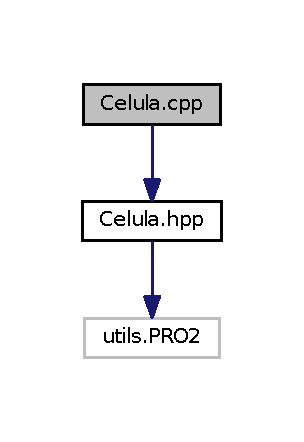
\includegraphics[width=146pt]{_celula_8cpp__incl}
\end{center}
\end{figure}


\subsection{Descripción detallada}
Código de la clase \hyperlink{class_celula}{Celula}. 

Definición en el archivo \hyperlink{_celula_8cpp_source}{Celula.\-cpp}.


\hypertarget{_celula_8hpp}{\section{Referencia del Archivo Celula.\-hpp}
\label{_celula_8hpp}\index{Celula.\-hpp@{Celula.\-hpp}}
}


Especificación de la clase \hyperlink{class_celula}{Celula}.  


Dependencia gráfica adjunta para Celula.\-hpp\-:\nopagebreak
\begin{figure}[H]
\begin{center}
\leavevmode
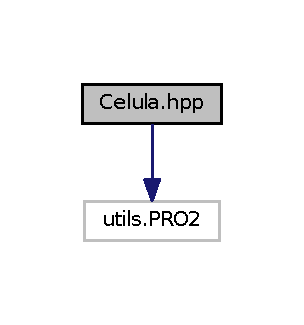
\includegraphics[width=146pt]{_celula_8hpp__incl}
\end{center}
\end{figure}
\subsection*{Clases}
\begin{DoxyCompactItemize}
\item 
class \hyperlink{class_celula}{Celula}
\begin{DoxyCompactList}\small\item\em Representa una celula con atributos identificador y actividad. \end{DoxyCompactList}\end{DoxyCompactItemize}


\subsection{Descripción detallada}
Especificación de la clase \hyperlink{class_celula}{Celula}. 

Definición en el archivo \hyperlink{_celula_8hpp_source}{Celula.\-hpp}.


\hypertarget{_experiment_8cpp}{\section{Referencia del Archivo Experiment.\-cpp}
\label{_experiment_8cpp}\index{Experiment.\-cpp@{Experiment.\-cpp}}
}


Código de la clase \hyperlink{class_experiment}{Experiment}.  


Dependencia gráfica adjunta para Experiment.\-cpp\-:\nopagebreak
\begin{figure}[H]
\begin{center}
\leavevmode
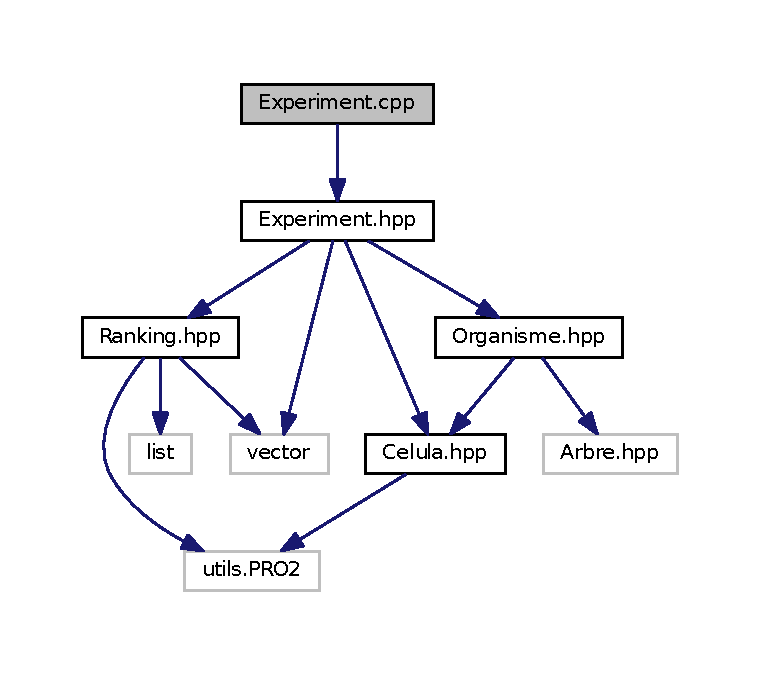
\includegraphics[width=350pt]{_experiment_8cpp__incl}
\end{center}
\end{figure}


\subsection{Descripción detallada}
Código de la clase \hyperlink{class_experiment}{Experiment}. 

Definición en el archivo \hyperlink{_experiment_8cpp_source}{Experiment.\-cpp}.


\hypertarget{_experiment_8hpp}{\section{Referencia del Archivo Experiment.\-hpp}
\label{_experiment_8hpp}\index{Experiment.\-hpp@{Experiment.\-hpp}}
}


Especificación de la clase \hyperlink{class_experiment}{Experiment}.  


Dependencia gráfica adjunta para Experiment.\-hpp\-:\nopagebreak
\begin{figure}[H]
\begin{center}
\leavevmode
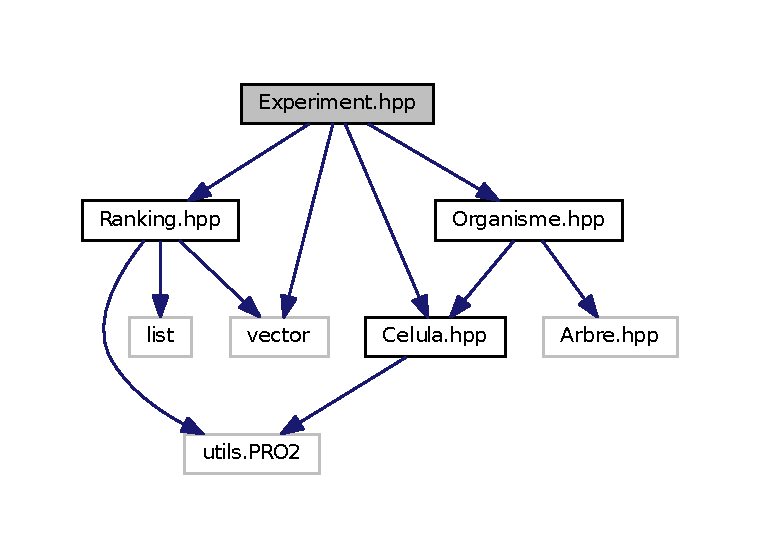
\includegraphics[width=350pt]{_experiment_8hpp__incl}
\end{center}
\end{figure}
\subsection*{Clases}
\begin{DoxyCompactItemize}
\item 
class \hyperlink{class_experiment}{Experiment}
\begin{DoxyCompactList}\small\item\em Representa un experiment como un conjunto de organismes. \end{DoxyCompactList}\end{DoxyCompactItemize}


\subsection{Descripción detallada}
Especificación de la clase \hyperlink{class_experiment}{Experiment}. 

Definición en el archivo \hyperlink{_experiment_8hpp_source}{Experiment.\-hpp}.


\hypertarget{_organisme_8cpp}{\section{Referencia del Archivo Organisme.\-cpp}
\label{_organisme_8cpp}\index{Organisme.\-cpp@{Organisme.\-cpp}}
}


Código de la clase \hyperlink{class_organisme}{Organisme}.  


Dependencia gráfica adjunta para Organisme.\-cpp\-:\nopagebreak
\begin{figure}[H]
\begin{center}
\leavevmode
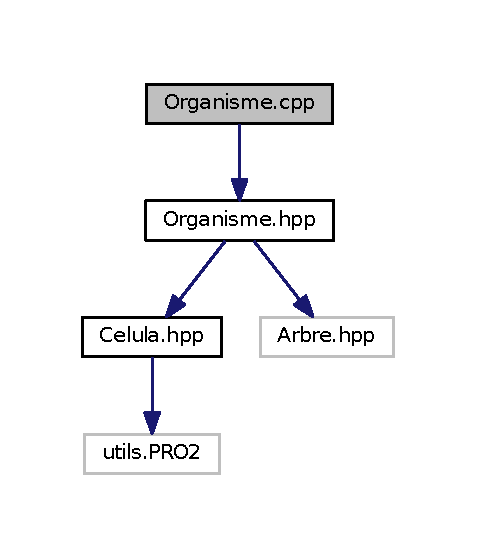
\includegraphics[width=229pt]{_organisme_8cpp__incl}
\end{center}
\end{figure}


\subsection{Descripción detallada}
Código de la clase \hyperlink{class_organisme}{Organisme}. 

Definición en el archivo \hyperlink{_organisme_8cpp_source}{Organisme.\-cpp}.


\hypertarget{_organisme_8hpp}{\section{Referencia del Archivo Organisme.\-hpp}
\label{_organisme_8hpp}\index{Organisme.\-hpp@{Organisme.\-hpp}}
}


Especificación de la clase \hyperlink{class_organisme}{Organisme}.  


Dependencia gráfica adjunta para Organisme.\-hpp\-:\nopagebreak
\begin{figure}[H]
\begin{center}
\leavevmode
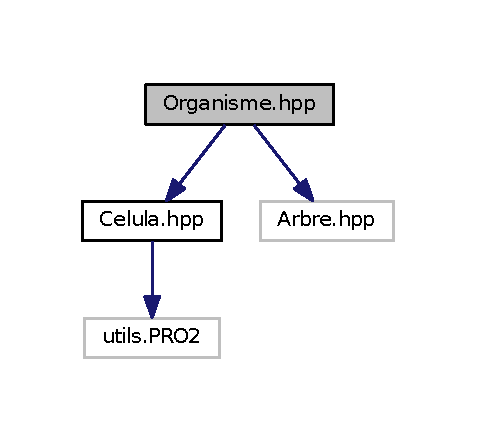
\includegraphics[width=229pt]{_organisme_8hpp__incl}
\end{center}
\end{figure}
\subsection*{Clases}
\begin{DoxyCompactItemize}
\item 
class \hyperlink{class_organisme}{Organisme}
\begin{DoxyCompactList}\small\item\em Representa un organisme como arbol de celulas, el máximo identificador y si puede crecer o no. \end{DoxyCompactList}\end{DoxyCompactItemize}


\subsection{Descripción detallada}
Especificación de la clase \hyperlink{class_organisme}{Organisme}. 

Definición en el archivo \hyperlink{_organisme_8hpp_source}{Organisme.\-hpp}.


\hypertarget{pro2_8cpp}{\section{Referencia del Archivo pro2.\-cpp}
\label{pro2_8cpp}\index{pro2.\-cpp@{pro2.\-cpp}}
}


Programa principal para la P\-R\-A\-C\-T\-I\-C\-A de P\-R\-O2.  


Dependencia gráfica adjunta para pro2.\-cpp\-:\nopagebreak
\begin{figure}[H]
\begin{center}
\leavevmode
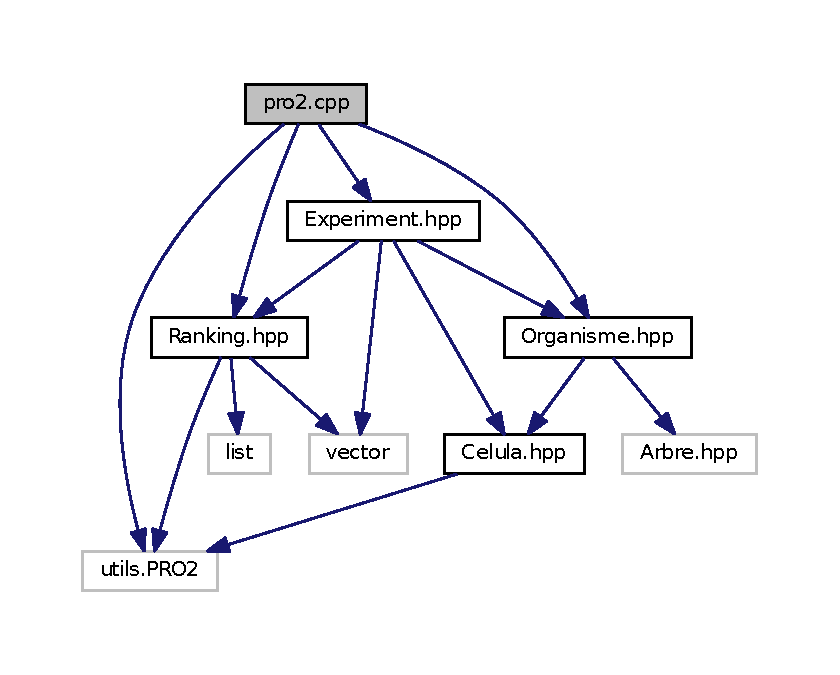
\includegraphics[width=350pt]{pro2_8cpp__incl}
\end{center}
\end{figure}
\subsection*{Funciones}
\begin{DoxyCompactItemize}
\item 
int \hyperlink{pro2_8cpp_ae66f6b31b5ad750f1fe042a706a4e3d4}{main} ()
\begin{DoxyCompactList}\small\item\em Programa principal para la P\-R\-A\-C\-T\-I\-C\-A de P\-R\-O2. \end{DoxyCompactList}\end{DoxyCompactItemize}


\subsection{Descripción detallada}
Programa principal para la P\-R\-A\-C\-T\-I\-C\-A de P\-R\-O2. 

Definición en el archivo \hyperlink{pro2_8cpp_source}{pro2.\-cpp}.



\subsection{Documentación de las funciones}
\hypertarget{pro2_8cpp_ae66f6b31b5ad750f1fe042a706a4e3d4}{\index{pro2.\-cpp@{pro2.\-cpp}!main@{main}}
\index{main@{main}!pro2.cpp@{pro2.\-cpp}}
\subsubsection[{main}]{\setlength{\rightskip}{0pt plus 5cm}int main (
\begin{DoxyParamCaption}
{}
\end{DoxyParamCaption}
)}}\label{pro2_8cpp_ae66f6b31b5ad750f1fe042a706a4e3d4}


Programa principal para la P\-R\-A\-C\-T\-I\-C\-A de P\-R\-O2. 



Definición en la línea 49 del archivo pro2.\-cpp.


\begin{DoxyCode}
\{
  \textcolor{comment}{// leer los valores enteros N (población inicial del experimento, mayor que
       1)}
  \textcolor{keywordtype}{int} N = readint();
  
  \textcolor{comment}{// leer M (máximo permitido de población histórica, mayor que N).}
  \textcolor{keywordtype}{int} M = readint();

  \textcolor{comment}{// leer los N organismos iniciales. Cada organismo ha de tener al }
  \textcolor{comment}{// menos una célula (es decir, ha de estar vivo).}
  \hyperlink{class_experiment}{Experiment} exp(M);
  \hyperlink{class_ranking}{Ranking} R(N,M);
  \textcolor{keywordtype}{int} fills\_ronda;
  exp.leer\_experiment(N);
  
  \textcolor{keywordtype}{int} op = readint();
  \textcolor{keywordflow}{while} (op != -6 and exp.tamano() < exp.tamano\_maximo() and not exp.muerto()) 
      \{
    \textcolor{keywordflow}{if} (op == -1) \{
      \textcolor{comment}{// Aplicar un estirón a un subconjunto de organismos. Se proporciona una}
      \textcolor{comment}{// secuencia de enteros no repetidos entre 1 y M.  Los organismos que
       estén}
      \textcolor{comment}{// vivos (y no hayan empezado a sufrir recortes) en el momento de
       realizar la}
      \textcolor{comment}{// tarea, cuyos identificadores estén en la secuencia, sufrirán el}
      \textcolor{comment}{// correspondiente estirón.}
      \textcolor{keywordtype}{int} x = readint();
      \textcolor{keywordflow}{for} (\textcolor{keywordtype}{int} i = 0; i < x; ++i) \{
        \textcolor{keywordtype}{int} y = readint();
        exp.estiron(y);
      \}
    \}
    
    \textcolor{keywordflow}{else} \textcolor{keywordflow}{if} (op == -2) \{
      \textcolor{comment}{// Aplicar un recorte a un subconjunto de organismos. Se proporciona una}
      \textcolor{comment}{// secuencia de enteros no repetidos entre 1 y M.  Los organismos que
       estén}
      \textcolor{comment}{// vivos en el momento de realizar la tarea, cuyos identificadores estén
       en la}
      \textcolor{comment}{// secuencia, sufrirán el correspondiente recorte.}
      \textcolor{keywordtype}{int} x = readint();
      \textcolor{keywordflow}{for} (\textcolor{keywordtype}{int} i = 0; i < x; ++i) \{
        \textcolor{keywordtype}{int} y = readint();
        exp.recorte(y);
      \}
    \}
    
    \textcolor{keywordflow}{else} \textcolor{keywordflow}{if} (op == -3) \{
      \textcolor{comment}{// Aplicar una ronda de reproducción a todos los organismos. Actualizar
       el}
      \textcolor{comment}{// ranking consecuentemente. Escribir el número de hijos nacidos en la
       ronda.}
      cout << \textcolor{stringliteral}{"RONDA DE EMPAREJAMIENTOS"} << endl;
      fills\_ronda = exp.reproduccion(R);
      cout << \textcolor{stringliteral}{"Nuevos organismos : "} << fills\_ronda << endl;
      cout << endl;
    \}
    
    \textcolor{keywordflow}{else} \textcolor{keywordflow}{if} (op == -4) \{
      \textcolor{comment}{// Obtener el ranking de reproducción de los organismos. Para cada
       organismo,}
      \textcolor{comment}{// vivo o muerto, que haya existido hasta el momento de la consulta se ha
       de}
      \textcolor{comment}{// obtener un listado de sus emparejamientos que hayan producido hijos. 
       Cada}
      \textcolor{comment}{// emparejamiento estará representado por el identificador de su
       compañero y el}
      \textcolor{comment}{// del hijo. El listado vendrá ordenado por el identificador de los
       hijos.}
      cout << \textcolor{stringliteral}{"RANKING"} << endl;
      R.escribir\_ranking();
      cout << endl;
    \}
    
    \textcolor{keywordflow}{else} \textcolor{keywordflow}{if} (op == -5) \{
      \textcolor{comment}{// Consultar el estado de un subconjunto de organismos. Se proporciona
       una}
      \textcolor{comment}{// secuencia de enteros no repetidos entre 1 y M.  Se escribirá la
       estructura}
      \textcolor{comment}{// celular de los organismos existentes (vivos o muertos) en el momento
       de}
      \textcolor{comment}{// realizar la tarea cuyos identificadores estén en la secuencia.}
      \textcolor{keywordtype}{int} x = readint();
      cout << \textcolor{stringliteral}{"ORGANISMOS"} << endl;
      \textcolor{keywordflow}{for} (\textcolor{keywordtype}{int} i = 0; i < x; ++i) \{
        \textcolor{keywordtype}{int} y = readint();
        exp.escribir\_organisme(y);
      \}
      cout << endl;
    \}
    
    \textcolor{keywordflow}{if} (exp.tamano() < exp.tamano\_maximo() or not exp.muerto()) op = readint();
  \}

  cout << \textcolor{stringliteral}{"FIN"} << endl;
  cout << endl;
  
  \textcolor{comment}{// Tras el fin del proceso, se ha de indicar la causa. }
  \textcolor{comment}{// Si ha sido porque la población ha llegado a M organismos (máximo}
  \textcolor{comment}{// permitido), se han de realizar dos consultas adicionales:}
  \textcolor{comment}{// Obtener el ranking}
  \textcolor{comment}{// Consultar el estado de los organismos nacidos en la última ronda de}
  \textcolor{comment}{// reproducción (atención: ésta ha podido ser incompleta)}
  
  cout << \textcolor{stringliteral}{"Organismos en total : "} << exp.tamano() << endl;
  cout << \textcolor{stringliteral}{"Organismos vivos : "} << exp.consultar\_vius() << endl;
  cout << endl;

  \textcolor{keywordflow}{if} (exp.tamano() == exp.tamano\_maximo()) \{
    cout << \textcolor{stringliteral}{"ORGANISMOS"} << endl;
    exp.escribir\_ultims(fills\_ronda);
    cout << endl;
    cout << \textcolor{stringliteral}{"RANKING"} << endl;
    R.escribir\_ranking();
  \}
\}
\end{DoxyCode}

\hypertarget{_ranking_8cpp}{\section{Referencia del Archivo Ranking.\-cpp}
\label{_ranking_8cpp}\index{Ranking.\-cpp@{Ranking.\-cpp}}
}


Código de la clase \hyperlink{class_ranking}{Ranking}.  


Dependencia gráfica adjunta para Ranking.\-cpp\-:\nopagebreak
\begin{figure}[H]
\begin{center}
\leavevmode
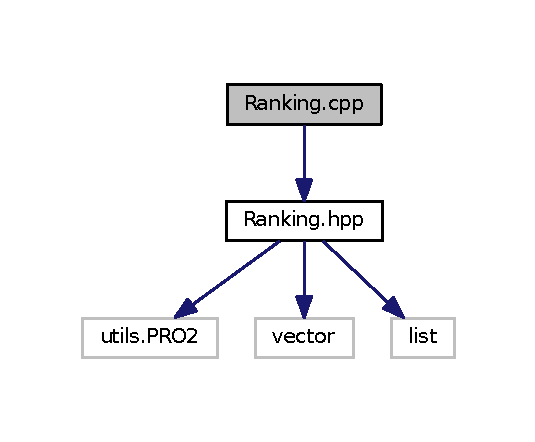
\includegraphics[width=257pt]{_ranking_8cpp__incl}
\end{center}
\end{figure}


\subsection{Descripción detallada}
Código de la clase \hyperlink{class_ranking}{Ranking}. 

Definición en el archivo \hyperlink{_ranking_8cpp_source}{Ranking.\-cpp}.


\hypertarget{_ranking_8hpp}{\section{Referencia del Archivo Ranking.\-hpp}
\label{_ranking_8hpp}\index{Ranking.\-hpp@{Ranking.\-hpp}}
}


Especificación de la clase \hyperlink{class_ranking}{Ranking}.  


Dependencia gráfica adjunta para Ranking.\-hpp\-:\nopagebreak
\begin{figure}[H]
\begin{center}
\leavevmode
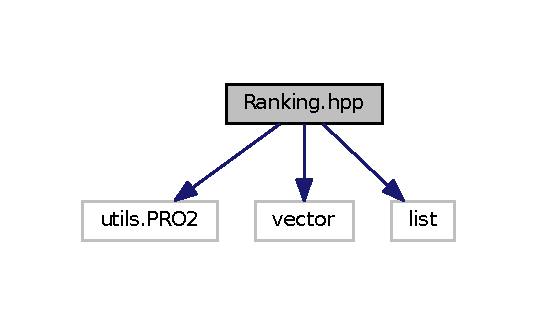
\includegraphics[width=257pt]{_ranking_8hpp__incl}
\end{center}
\end{figure}
\subsection*{Clases}
\begin{DoxyCompactItemize}
\item 
class \hyperlink{class_ranking}{Ranking}
\begin{DoxyCompactList}\small\item\em Representa un ranking de todos los organismos del experiment. \end{DoxyCompactList}\end{DoxyCompactItemize}


\subsection{Descripción detallada}
Especificación de la clase \hyperlink{class_ranking}{Ranking}. 

Definición en el archivo \hyperlink{_ranking_8hpp_source}{Ranking.\-hpp}.


\addcontentsline{toc}{part}{Índice}
\printindex
\end{document}
